\documentclass[a4paper]{article}
\usepackage[T1]{fontenc}			% pacchetto per \chapter
\usepackage[italian]{babel}
\usepackage[italian]{isodate}  		% formato delle date in italiano
\usepackage{graphicx}				% gestione delle immagini
\usepackage{amsfonts}
\usepackage{booktabs}				% tabelle di qualità superiore
\usepackage{amsmath}				% pacchetto matematica
\usepackage{enumitem}				% gestione delle liste
\usepackage{pifont}					% pacchetto con elenchi carini
\usepackage{listings}				% pacchetto per i codici
\usepackage[x11names]{xcolor}		% pacchetto colori RGB
% Link ipertestuali per l'indice
\usepackage{xcolor}
\usepackage[linkcolor=black, citecolor=blue, urlcolor=cyan]{hyperref}
\hypersetup{
	colorlinks=true
}

\newcommand{\longline}{\noindent\rule{\textwidth}{0.4pt}}

\definecolor{codegreen}{rgb}{0,0.6,0}
\definecolor{codegray}{rgb}{0.5,0.5,0.5}
\definecolor{codepurple}{rgb}{0.58,0,0.82}
\definecolor{backcolour}{rgb}{0.95,0.95,0.92}
\lstdefinestyle{mystyle}{
	backgroundcolor=\color{backcolour},   
	commentstyle=\color{codegreen},
	keywordstyle=\color{magenta},
	numberstyle=\tiny\color{codegray},
	stringstyle=\color{codepurple},
	basicstyle=\ttfamily\footnotesize,
	breakatwhitespace=false,         
	breaklines=true,                 
	captionpos=b,                    
	keepspaces=true,                 
	numbers=left,                    
	numbersep=5pt,                  
	showspaces=false,                
	showstringspaces=false,
	showtabs=false,                  
	tabsize=2
}

\lstdefinelanguage{JavaScript}{
	keywords={typeof, new, true, false, catch, function, return, null, catch, switch, var, if, in, while, do, else, case, break},
	keywordstyle=\color{blue}\bfseries,
	ndkeywords={class, export, boolean, throw, implements, import, this},
	ndkeywordstyle=\color{darkgray}\bfseries,
	identifierstyle=\color{black},
	sensitive=false,
	comment=[l]{//},
	morecomment=[s]{/*}{*/},
	commentstyle=\color{codegreen}\ttfamily,
	stringstyle=\color{red}\ttfamily,
	morestring=[b]',
	morestring=[b]"
}

\lstset{
	language=JavaScript,
	backgroundcolor=\color{lightgray},
	extendedchars=true,
	basicstyle=\footnotesize\ttfamily,
	showstringspaces=false,
	showspaces=false,
	numbers=left,
	numberstyle=\footnotesize,
	numbersep=9pt,
	tabsize=2,
	breaklines=true,
	showtabs=false,
	captionpos=b
}

\lstset{style=mystyle}

%\usepackage{showframe}				% visualizzazione bordi
%\usepackage{showkeys}				% visualizzazione etichetta

\newcommand{\dquotes}[1]{``#1''}

\begin{document}
	\author{VR443470}
	\title{Programmazione e sicurezza delle reti}
	\date{\printdayoff\today}
	\maketitle
	
	\newpage
	
	% indice
	\tableofcontents
	
	\newpage
	
	\section{Scrittura di applicazioni di rete mediante interfaccia socket}
	
	\subsection{Host, processo e applicazione}
	
	L'\textcolor{Red3}{\textbf{host}} (colui che ospita) è una \textbf{macchina} sempre identificata da un indirizzo IP a cui, opzionalmente, può essere associato un nome Internet.\newline
	
	\noindent
	Il \textcolor{Red3}{\textbf{processo}} è un \textbf{programma in esecuzione} sull'host, il quale trasmette/riceve pacchetti verso/da altri processi su altri host attraverso la rete. Viene identificato tramite un numero di porta nell'intervallo $0$ - $65535$.\newline
	
	\noindent
	Un \textcolor{Red3}{\textbf{applicazione}} è una collaborazione tra un \textbf{insieme di processi} sparsi sulla rete per fare qualcosa di utile per l'utente, per esempio chat, e-mail, ecc.\newline
	
	\noindent
	Alcuni \textcolor{Green4}{\textbf{esempi}}:
	\begin{itemize}
		\item Eseguendo una ricerca su internet:
		\begin{itemize}
			\item Il \emph{web} è l'applicazione;
			\item Mentre i browser (Chrome, Firefox, Edge, Safari) sono il processo di esecuzione;
			\item L'host è il PC, tablet o smartphone su cui viene aperto il browser;
			\item Apache o NGINX è il processo di esecuzione sulla macchina remota, anch'essa identificata come host.
		\end{itemize}
		
		\item Aprendo un'applicazione come Telegram:
		\begin{itemize}
			\item Telegram è l'applicazione;
			\item Il processo di esecuzione è sempre l'app Telegram che è in esecuzione sul dispositivo attualmente in uso (PC, tablet, ecc.) che funge da host;
			\item Il server di Telegram è il processo di esecuzione sulla macchina remota, anch'essa identificata come host.
		\end{itemize}
	\end{itemize}\newpage

	\subsection{Modalità di trasmissione in Internet}
	
	Su Internet la modalità di trasmissione è una sequenza di byte chiamata: pacchetto, Protocol Data Unit (PDU), Datagram. A seconda del livello del protocollo, ci sono nomi diversi.
	
	\longline
	
	\subsubsection{Applicazioni orientate al datagramma (UDP)}
	
	Alcune \textbf{applicazioni sono orientate al datagramma}, quindi \textbf{ogni pacchetto scambiato tra gli host è indipendente dai precedenti e successivi}. Le \textbf{perdite} di pacchetti non vengono tenute in considerazione ed un \textcolor{Green4}{\textbf{esempio}} può essere la \textbf{trasmissione di temperature}: il ricevitore può non tener conto di alcune perdite poiché le informazioni ricevute non sono necessarie per il futuro.
	
	\longline
	
	\subsubsection{Applicazioni orientate alla connessione (TCP)}
	
	Invece, alcune \textbf{applicazioni sono orientate alla connessione}. A differenza delle applicazioni orientate al datagramma, quelle orientate alla connessione devono tener conto delle perdite poiché solitamente le informazioni scambiate sono di dimensioni rilevanti (e.g. un'immagine). Di conseguenza, una perdita provocherebbe una lettura parziale o impossibile da parte del ricevitore.\newline
	
	\noindent
	Il \textbf{socket} si preoccupa di \textbf{numerare i pacchetti appartenenti alla stessa connessione} per rilevare eventuali pacchetti persi e poterli ritrasmettere.\newline
	
	\noindent
	Il sistema operativo introduce all'interno dei pacchetti un numero di sequenza così che possa rilevare eventuali pacchetti persi e ritrasmetterli.
	\begin{itemize}
		\item \textcolor{Green4}{\textbf{Vantaggi:}}
		\begin{itemize}
			\item L'utente scrive/legge su un archivio remoto con la stessa naturalezza di quando scrive/legge su un archivio locale come se la rete in mezzo non ci fosse.
		\end{itemize}
		
		\item \textcolor{Red3}{\textbf{Svantaggi:}}
		\begin{itemize}
			\item Gli host mittente e destinatario eseguono un lavoro più complesso con il sistema operativo;
			\item Ritardo di ritrasmissione nel caso in cui i pacchetti vengano persi.
		\end{itemize}
	\end{itemize}\newpage

	\subsection{Schemi di applicazioni che utilizzano la rete}
	
	Le applicazioni di rete sono insiemi di processi su host diversi che si scambiano messaggi attraverso la rete. \textbf{Esistono degli schemi base che regolano lo scambio di messaggi}:
	\begin{itemize}
		\item Modello client/server;
		\item Modello Publisher/Subscriber (Pub/Sub)
	\end{itemize}

	\longline
	
	\subsubsection{Modello client/server}
	
	Il \textcolor{Red3}{\textbf{modello client/server}} è quello più utilizzato e funziona nel seguente modo (attenzione all'ordine!):
	\begin{enumerate}
		\item Il \emph{client} esegue una \textbf{richiesta} inviando dei dati al \emph{server};
		
		\item Il \emph{server} riceve i dati del \emph{client}, processa i dati e invia la \textbf{risposta} al \emph{client}. Infine, si mette in attesa di altre richieste.
	\end{enumerate}
	I dati inviati dal \emph{client} possono essere delle trasmissioni di dati o delle richieste di dati. In ogni caso, \textbf{il ruolo è determinato dall'ordine dei messaggi e non dal contenuto}. Si noti che il \emph{client} e \emph{server} \textbf{sono processi e \underline{non host}}. Infatti, l'insieme di un client e un server costituisce l'applicazione di rete.\newline
	
	\noindent
	Un \textcolor{Green4}{\textbf{esempio}} di applicazione client/server è il \textbf{sensore di temperatura corporea} che funge da client e invia al server una temperatura. Le risposte del server sono \dquotes{OK} per confermare l'avvenuta ricezione.\newline
	
	\noindent
	Un altro \textcolor{Green4}{\textbf{esempio}} di applicazione client/server è il display che funge da cliente e chiede al server una temperatura. Le risposte del server in questo caso saranno i dati richiesti.
	
	\longline
	
	\subsection{Creazione dell'interfaccia Socket}
	
	Il programma, prima di utilizzare la rete, deve essere in grado di creare un oggetto di tipo \textbf{socket}. Esso è identificato principalmente da tre parametri:
	\begin{itemize}
		\item Indirizzo IP locale;
		
		\item Porta locale, la quale è un intero senza segno di 16 bit (quindi da 0 a 65'535). Nel modello client/server:
		\begin{itemize}
			\item Il \textbf{server} deve decidere esplicitamente il numero di porta affinché i client possano saperlo (da 0 a 1023 le porte sono chiamate \dquotes{porte note} perché sono utilizzate per protocolli famosi come HTTP);
			
			\item Il \textbf{client} può decidere se scegliere il numero di porta esplicitamente oppure delegare la scelta al sistema operativo.
		\end{itemize}

		\item Modalità di trasmissione: UDP o TCP.
	\end{itemize}\newpage
	
	\subsection[\textcolor{Green4}{\textbf{Esempi}} di codice]{Esempi di codice}
	
	\subsubsection{Esecuzione degli esempi}
	
	\begin{enumerate}
		\item Aprire due terminali
		
		\item Compilare il server e successivamente eseguirlo con il comando:
		\begin{lstlisting}[language=C]
			-gcc network.c serverUDP.c -o serverUDP -lpthread\end{lstlisting}
		
		\item Compilare il client e successivamente eseguirlo con il comando:
		\begin{lstlisting}[language=C]
			-gcc network.c clientUDP.c -o clientUDP -lpthread\end{lstlisting}
	\end{enumerate}

	\longline
	
	\subsubsection{Client UDP}\label{client UDP}
	
	Il client UDP ha il seguente codice:
	\lstinputlisting[language=C]{code/clientUDP.c}
	\begin{itemize}
		\item (4-8) dichiarazione delle variabili tra cui la variabile socket;
	
		\item (10) inizializzazione dell'interfaccia socket sulla porta 20'000;
	
		\item (13) invio, tramite UDP, il messaggio \dquotes{Ciao sono il client!} al destinatario avente indirizzo IP \dquotes{127.0.0.1} (\emph{localhost}) e porta 35'000;
	
		\item (14) attesta dell'arrivo della risposta del server;
		
		\item (15-16) scrittura sul terminale della porta, dell'indirizzo del mittente e del messaggio.
	\end{itemize}\newpage
	
	\subsubsection{Server UDP}\label{server UDP}
	
	Il server UDP ha il seguente codice:
	\lstinputlisting[language=C]{code/serverUDP.c}
	\begin{itemize}
		\item (4-8) dichiarazione delle variabili tra cui la variabile socket;
		
		\item (10) inizializzazione dell'interfaccia socket sulla porta 35'000;
		
		\item (12) attesta dell'arrivo di qualche messaggio da parte di qualche client;
		
		\item (13-14) ricezione di un messaggio da parte di un client e stampa sul terminale dell'indirizzo, della porta e del messaggio del mittente;
		
		\item (15) invio della risposta del server al client.
	\end{itemize}\newpage

	\subsubsection{Client\_inc UDP}\label{client_inc UDP}
	
	Il client UDP (paragrafo~\ref{client UDP}) può essere riscritto nel seguente modo:
	\lstinputlisting[language=C]{code/clientUDP_inc.c}
	\begin{itemize}
		\item (4-8) dichiarazione delle variabili tra cui la variabile socket;
		
		\item (10) inizializzazione dell'interfaccia socket sulla porta 20'000;
		
		\item (11-12) inserimento di un numero intero da parte dell'utente;
		
		\item (13) invio, tramite UDP, del numero inserito dall'utente al destinatario avente indirizzo IP \dquotes{127.0.0.1} (\emph{localhost}) e porta 35'000;
		
		\item (14) attesta dell'arrivo della risposta del server;
		
		\item (15-16) scrittura sul terminale della porta, dell'indirizzo del mittente e del messaggio.
	\end{itemize}\newpage

	\subsubsection{Server\_inc UDP}\label{server_inc UDP}
	
	Il server UDP (paragrafo~\ref{server UDP}) può essere riscritto nel seguente modo:
	\lstinputlisting[language=C]{code/serverUDP_inc.c}
	\begin{itemize}
		\item (4-8) dichiarazione delle variabili tra cui la variabile socket;
		
		\item (10) inizializzazione dell'interfaccia socket sulla porta 35'000;
		
		\item (12) attesta dell'arrivo di qualche messaggio da parte di qualche client;
		
		\item (13-14) ricezione di un messaggio da parte di un client e stampa sul terminale dell'indirizzo, della porta e del messaggio del mittente;
		
		\item (15) incremento di uno del valore intero ottenuto;
		
		\item (15) invio della risposta del server al client con il valore incrementato.
	\end{itemize}\newpage

	\subsubsection{Client TCP}\label{client TCP}
	
	Il client TCP ha il seguente codice:
	\lstinputlisting[language=C]{code/clientTCP.c}
	\begin{itemize}
		\item (4-5) dichiarazione delle variabili tra cui la variabile \textsf{connection} per gestire la connessione;
		
		\item (7-8) creazione di una connessione TCP con il server utilizzando \emph{localhost} e la porta 35'000. 
		
		\item (9-10) controllo del valore della connessione per verificare se c'è stato un errore. In tal caso, la connessione termina con la stampa dell'errore su terminale;
		
		\item (12-15) in caso di connessione riuscita, il client richiede l'inserimento di un valore intero all'utente;
		
		\item (16-17) invio del valore intero al server;
		
		\item (18) attesa di una risposta da parte del server;
		
		\item (19-20) al momento della ricezione della risposta, il client stampa la risposta del server e chiude la connessione.
	\end{itemize}\newpage
	
	\subsubsection{Server TCP}\label{server TCP}
	
	Il server TCP ha il seguente codice:
	\lstinputlisting[language=C]{code/serverTCP.c}
	\begin{itemize}
		\item (4-6) dichiarazione delle variabili tra cui la variabile \textsf{connection} per gestire la connessione e \textsf{socket} per gestire i dati;
		
		\item (8) inizializzazione di un socket TCP utilizzando la porta 35'000.
		
		\item (9-10) controllo del valore del socket per verificare se c'è stato un errore. In tal caso, la creazione termina con la stampa dell'errore su terminale;
		
		\item (12-14) in caso di creazione del socket riuscita, il server attende la connessione da parte di qualche client;
		
		\item (15-17) attesa di una richiesta da parte di qualche client. Nel momento in cui viene ricevuta una richiesta, il server la accetta e instaura la connessione e attende la ricezione dei dati;
		
		\item (18-19) all'arrivo dei dati da parte del client, il server esegue un incremento di uno del valore ricevuto dal client;
		
		\item (20-22) il server invia il valore al client e infine chiude la connessione.
	\end{itemize}\newpage

	\subsubsection{Codice per la copia di un file}
	
	Il codice per la copia di un file è strutturato nel seguente modo:
	\lstinputlisting[language=C]{code/fileCopy.c}
	\begin{itemize}
		\item (6-29) dichiarazione dei puntatori ai file e tentativi di apertura dei due file richiesti dall'utente;
		
		\item (32-37) viene eseguita la lettura dal primo file e salvata nella variabile \textsf{c}. A questo punto, finché viene letto un carattere valido, ovvero che non sia la fine del file (\emph{End Of File}, EOF), il contenuto della variabile \textsf{c} viene inserito nel secondo file;

		\item (39-43) al termine del processo di copia, viene stampato il file nel quale sono stati copiati i valori e chiusi i rispettivi file descriptors.
	\end{itemize}\newpage
	
	\subsection[\textcolor{Red3}{\textbf{Esercizi}}]{Esercizi}
	
	\subsubsection{Esercizio 1}
	
	Lanciare prima il server e poi il client. Cosa si osserva? Invertire la sequenza di lancio. Cosa si osserva?\newline
	
	\noindent
	\textcolor{Green4}{\textbf{\emph{\underline{Soluzione}}}}\newline
	
	\noindent
	Lanciando il server e successivamente il client, il primo attende la connessione da parte di qualcuno. Quindi, una volta avviato il client, le due parti inizieranno a comunicare.
	
	Invece, avviando prima il client e successivamente il server, le due parti non riescono a comunicare. Questo perché il client tenta di raggiungere un host non esistente.
	
	\longline
	
	\subsubsection{Esercizio 2}
	
	Modificare i sorgenti per consentire al server di ricevere sulla porta 10000 e il client di trasmettere sulla propria porta 30000 (ogni modifica dei sorgenti richiede una loro ricompilazione).\newline
	
	\noindent
	\textcolor{Green4}{\textbf{\emph{\underline{Soluzione}}}}\newline
	
	\noindent
	Le modifiche da effettuare sono banali, ecco qua di seguito i codici del client (spiegazione al paragrafo~\ref{client UDP}):
	\lstinputlisting[language=C]{code/clientUDP_mod2.c}\newpage
	
	\noindent
	E del server (spiegazione al paragrafo~\ref{server UDP}):
	\lstinputlisting[language=C]{code/serverUDP_mod2.c}
	
	\longline
	
	\subsubsection{Esercizio 3}
	
	Mettere il server in ascolto sulla porta 100 e osservare cosa succede:
	\begin{itemize}
		\item Bisogna modificare anche il client? Se sì, dove?
		\item Per chi usa il proprio PC con Linux o una virtual machine Linux, lanciare il server con il comando \dquotes{\textsf{sudo ./serverUDP}} e osservare cosa cambia.
	\end{itemize}

	\noindent
	\textcolor{Green4}{\textbf{\emph{\underline{Soluzione}}}}\newline
	
	\noindent
	Modificando il codice e inserendo il numero di porta 100, il server non riesce ad essere eseguito per un problema della porta. Infatti, la porta 100 fa parte delle \emph{well-know port} e non può essere utilizzata per altri scopi.\newline
	
	\noindent
	Modificando anche il client e inviando il messaggio al localhost con porta 100, il codice viene compilato ed eseguito correttamente. Ovviamente il client rimane in attesa del server.\newline
	
	\noindent
	Compilando il server con la modalità \textsf{sudo} è possibile forzare la modifica della porta 100 e mettersi in ascolto su tale porta. Di conseguenza, il server si metterà in ascolto sulla porta 100 e il client che eseguirà l'invio di un messaggio in tale porta, riuscirà a trasmettere il messaggio.\newpage
	
	\subsubsection{Esercizio 4}
	
	Sostituire \dquotes{127.0.0.1} (o la stringa \dquotes{localhost}) con localhost (o al contrario con 127.0.0.1) e poi con \dquotes{pippo} e osservare cosa succede.\newline
	
	\noindent
	\textcolor{Green4}{\textbf{\emph{\underline{Soluzione}}}}\newline
	
	\noindent
	Modificando il parametro della chiamata a funzione \textsf{UDPSend} nel client viene modificato l'indirizzo del destinatario:
	\begin{itemize}
		\item Inserendo \dquotes{127.0.0.1} si sta inserendo l'indirizzo privato creato per identificare l'host stesso;

		\item Inserendo \textsf{localhost} si sta utilizzando un \emph{alias}, dunque è come scrivere l'indirizzo \dquotes{127.0.0.1};

		\item Inserendo \dquotes{Pippo} si sta provando a identificare l'alias Pippo a qualche indirizzo. Purtroppo non esiste nessun alias all'interno del sistema operativo con tale valore, tuttavia su Linux (forse anche su Windows) è possibile creare alias di rete con il relativo indirizzo IP.
	\end{itemize}

	\longline
	
	\subsubsection{Esercizio 5}
	
	(Da fare solo se in Lab Delta) Accordarsi per lavorare su coppie di macchine in modo che server e client siano su macchine diverse. Come bisogna modificare i sorgenti?\newline
	
	\noindent
	\textcolor{Green4}{\textbf{\emph{\underline{Soluzione}}}}\newline
	
	\noindent
	La modifica è alquanto semplice. Supponendo che i due host siano connessi sulla stessa rete, quindi non per forza la rete universitaria ma va bene anche un hotspot tramite telefono, è necessario modificare nel seguente modo i codici:
	\begin{itemize}
		\item Server: non apportare nessuna modifica in quanto il server (destinatario) deve solo aprire una porta, nel caso d'esempio la 35000;
		
		\item Client: indipendentemente dalla porta aperta nel client, di default nell'esempio la 20000, il client necessita di una modifica nei parametri della chiamata a funzione \textsf{UDPSend}. In particolare, al posto di \textsf{localhost} o dell'indirizzo \dquotes{127.0.0.1}, basterà inserire l'indirizzo IP del server che ha all'interno della rete. È doveroso cambiare anche il numero di porta nel caso in cui sia stata cambiata nel server.
		
		Attenzione, nelle virtual machine non è così semplice la faccenda. Infatti esse utilizzano un bridge per collegarsi alla scheda di rete e di conseguenza l'IP che viene visualizzato non è \dquotes{reale}. Si consiglia dunque un sistema operativo linux (o windows) non virtualizzato.
	\end{itemize}\newpage
	
	\subsubsection{Esercizio 6}
	
	Modificare il server in maniera che soddisfi 5 richieste prima di terminare.
	\begin{itemize}
		\item E se volessi che non terminasse mai?
	\end{itemize}

	\noindent
	\textcolor{Green4}{\textbf{\emph{\underline{Soluzione}}}}\newline
	
	\noindent
	Per soddisfare almeno 5 richieste, è necessario modificare il codice del server di modo che esegua la parte di codice della ricezione almeno 5 volte. Quindi il relativo codice del server sarà:
	\lstinputlisting[language=C]{code/serverUDP_mod3.c}
	Mentre quello del client non viene modificato.
	
	\noindent
	La simulazione dell'esecuzione sarà la seguente (prossima pagina):
	\begin{figure}[!htp]
		\centering
		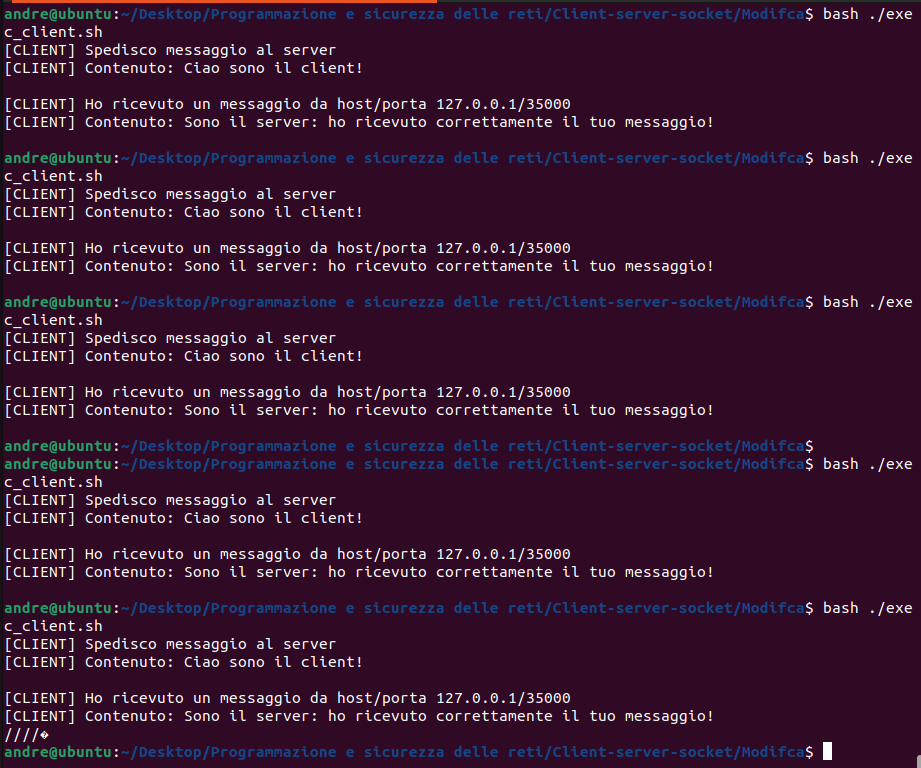
\includegraphics[width=\textwidth]{img/soluzioni_TCP-UDP/TCP-UDP_1.png}
		\caption{Terminale client.}
		\:\newline
		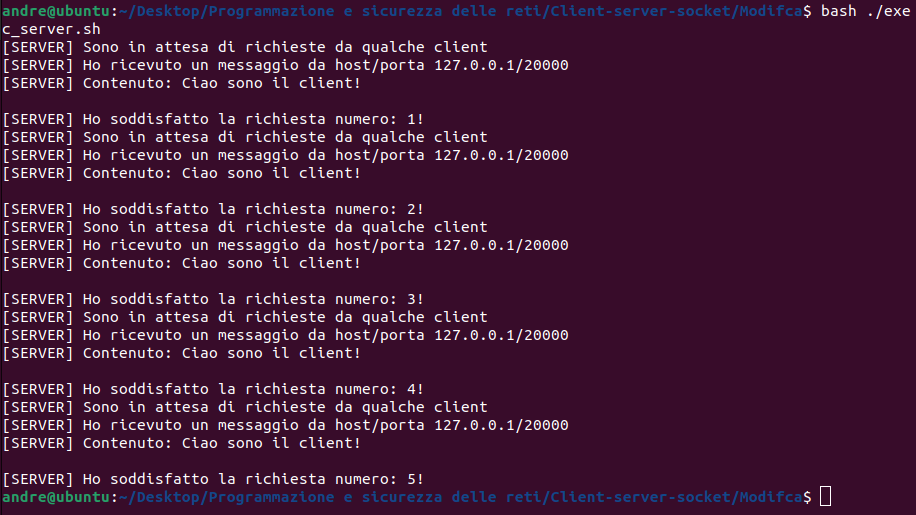
\includegraphics[width=\textwidth]{img/soluzioni_TCP-UDP/TCP-UDP_2.png}
		\caption{Terminale server.}
	\end{figure}\newpage

	\subsubsection{Esercizio 7}
	
	Compilare ed eseguire il secondo esempio.\newline
	
	\noindent
	\textcolor{Green4}{\textbf{\emph{\underline{Soluzione}}}}\newline
	
	\noindent
	Si esegue il secondo esempio che riguarda il clientUDP e serverUDP in versione \_inc, rispettivamente paragrafo~\ref{client_inc UDP} e \ref{server_inc UDP}.
	
	\longline
	
	\subsubsection{Esercizio 8}
	
	Modificare il codice in modo tale da costruire una semplice sommatrice:
	\begin{itemize}
		\item Il client acquisisce ripetutamente da tastiera un numero intero e lo invia al server finché l'utente digita zero;
		
		\item Il server accumula in una variabile \dquotes{somma} i valori mandati dal client finché il client manda zero;
		
		\item Quando il client manda zero il server risponde al client con la somma ottenuta.
	\end{itemize}

	\noindent
	\textcolor{Green4}{\textbf{\emph{\underline{Soluzione}}}}\newline
	
	\noindent
	Il codice del client:
	\lstinputlisting[language=C]{code/clientUDP_inc_mod2.c}
	\begin{itemize}
		\item 
		
		\item 
		
		\item 
	\end{itemize}
	\begin{figure}[!htp]
		\centering
		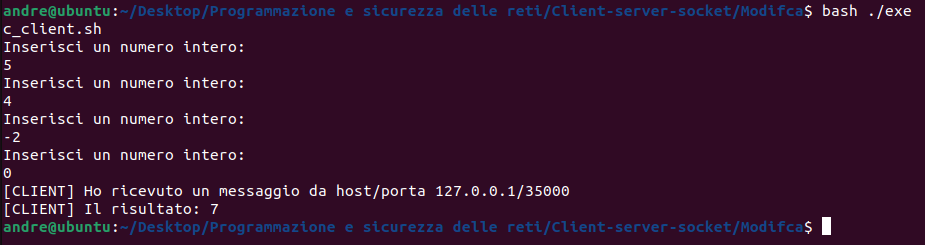
\includegraphics[width=\textwidth]{img/soluzioni_TCP-UDP/TCP-UDP_3.png}
		\caption{Esempio di esecuzione del client.}
	\end{figure}
	\newpage

	\noindent
	Il codice del server:
	\lstinputlisting[language=C]{code/serverUDP_inc_mod2.c}
	\begin{itemize}
		\item 
		
		\item 
		
		\item 
	\end{itemize}
	\begin{figure}[!htp]
		\centering
		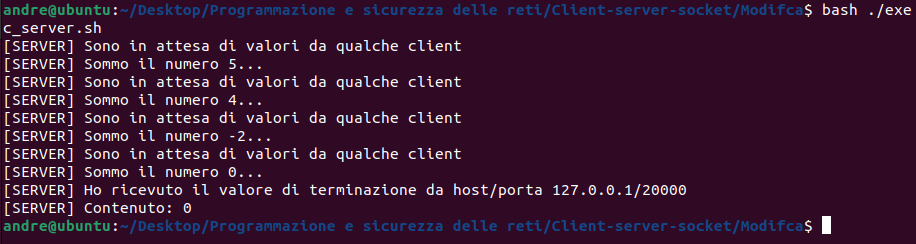
\includegraphics[width=\textwidth]{img/soluzioni_TCP-UDP/TCP-UDP_4.png}
		\caption{Esempio di esecuzione del server.}
	\end{figure}\newpage
	\:
	\newpage

	\section{Dal Web ai Webservices}
	
	\subsection{Protocollo HTTP/HTTPS}
	
	Il \textcolor{Red3}{\textbf{protocollo HTTP}} venne inventato per fruire dei contenuti in rete (\emph{World Wide Web}). Tuttavia, al giorno d'oggi viene usato per l'invocazione di funzionalità remote, tecnica chiamata \textbf{Webservice}.\newline
	
	\noindent
	Il protocollo si divide in più \textbf{fasi}:
	\begin{enumerate}
		\item Apertura di una connessione TCP;
		
		\item Nel caso del protocollo HTTPS, avviene l'autenticazione del server e negoziazione di una chiave di cifratura;
		
		\item Invio di messaggi di \emph{request} e \emph{response};
		
		\item Chiusura della connessione TCP.
	\end{enumerate}
	\begin{figure}[!htp]
		\centering
		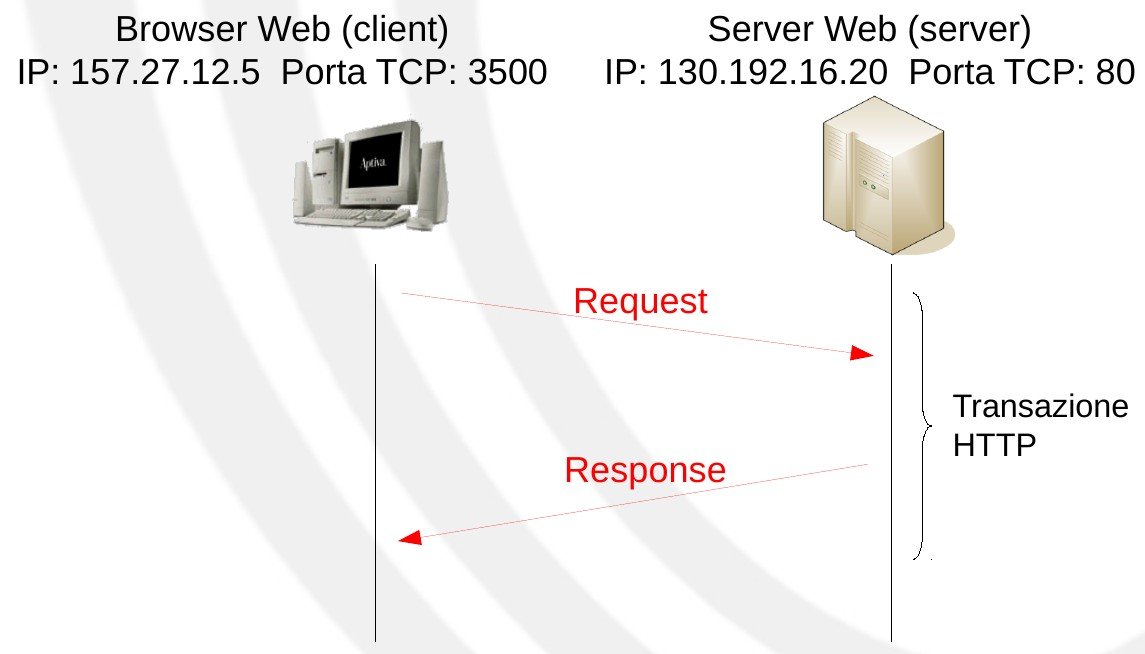
\includegraphics[width=\textwidth]{img/protocollo_http-https.png}
		\caption{Esempio di scambio di messaggi nel protocollo HTTP.}
	\end{figure}\newpage
	
	\noindent
	Nel \textcolor{Red3}{\textbf{protocollo HTTPS}} i messaggi che passano nella connessione TCP, sono gli stessi del protocollo HTTP con l'aggiunta di una \textbf{cifratura dei dati in transito} e di una \textbf{autenticazione del server mediante certificato digitale}. Inoltre, il server lavora sulla porta 443 e non sulla porta classica 80.
	\begin{figure}[!htp]
		\centering
		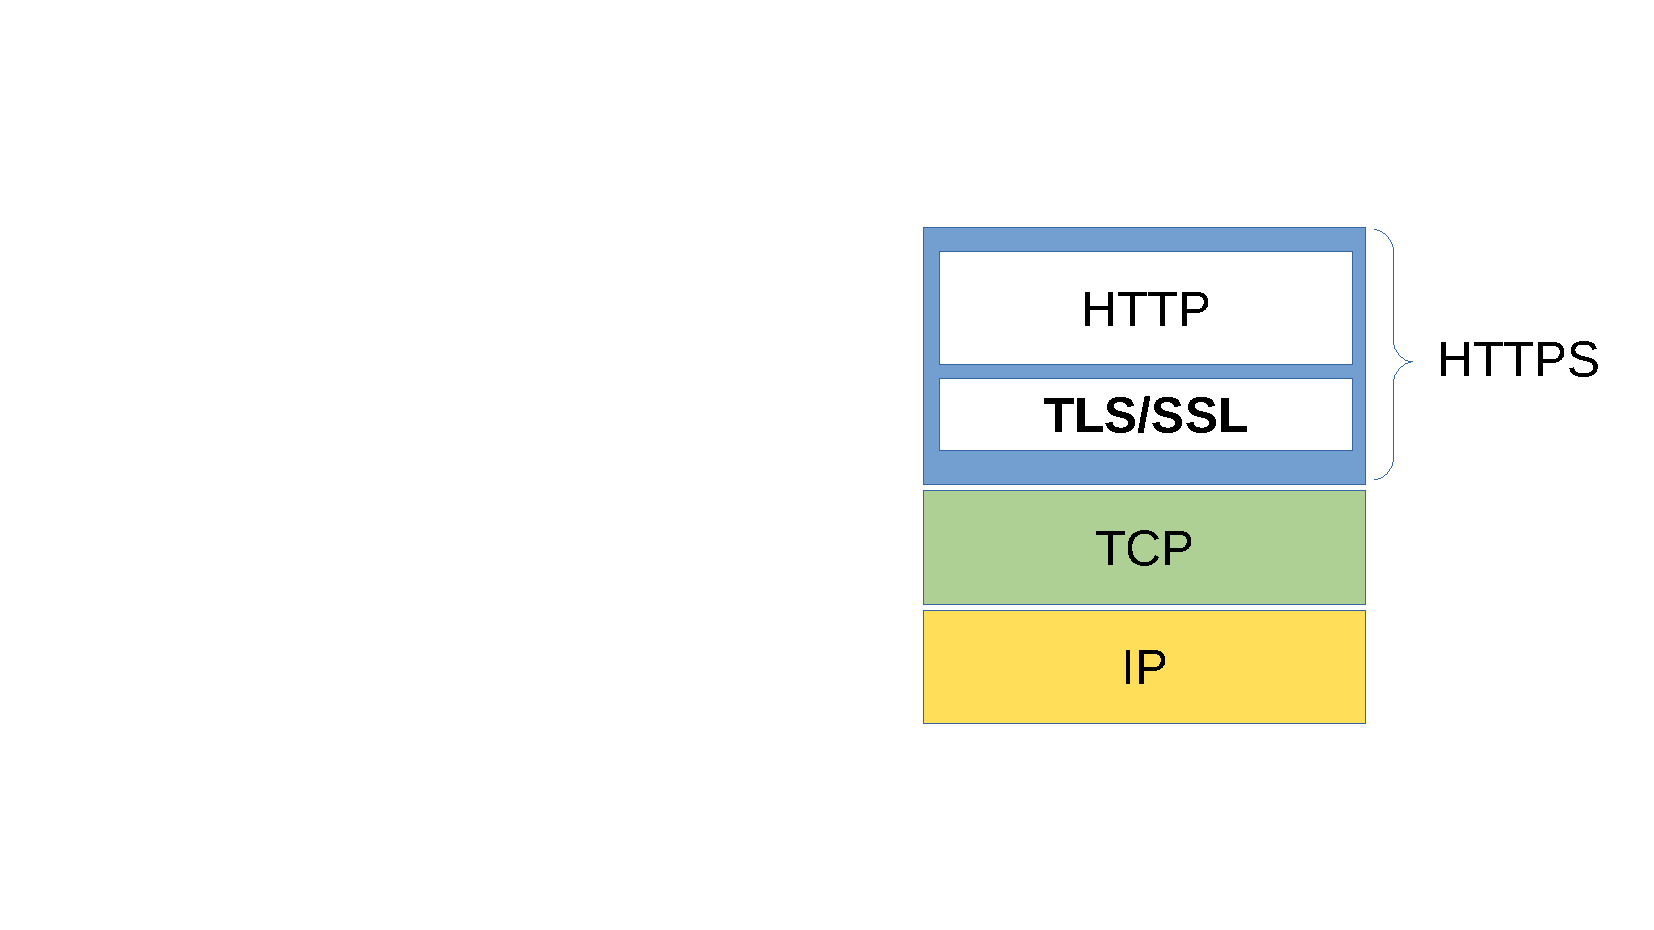
\includegraphics[width=.4\textwidth]{img/protocollo_https.pdf}
		\caption{Protocollo HTTPS.}
	\end{figure}

	\noindent
	Un \textcolor{Green4}{\textbf{esempio}} di richiesta:
	\begin{figure}[!htp]
		\centering
		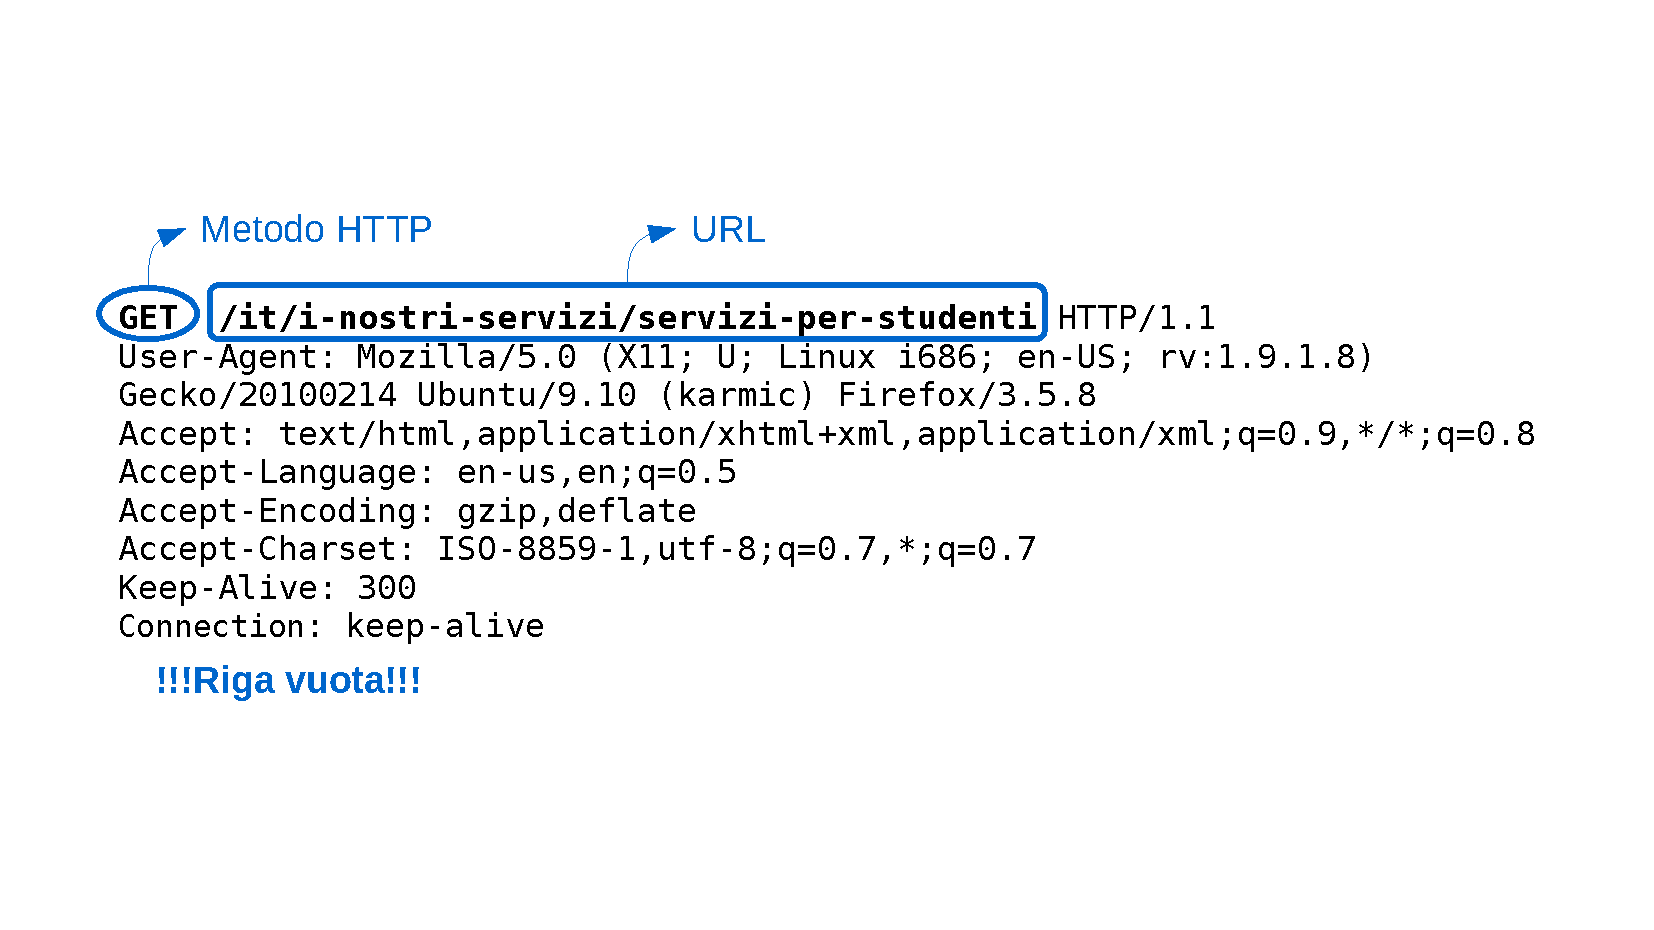
\includegraphics[width=\textwidth]{img/richiesta_http.pdf}
		\caption{Messaggio di richiesta.}
	\end{figure}

	\noindent
	Un \textcolor{Green4}{\textbf{esempio}} di risposta:
	\begin{figure}[!htp]
		\centering
		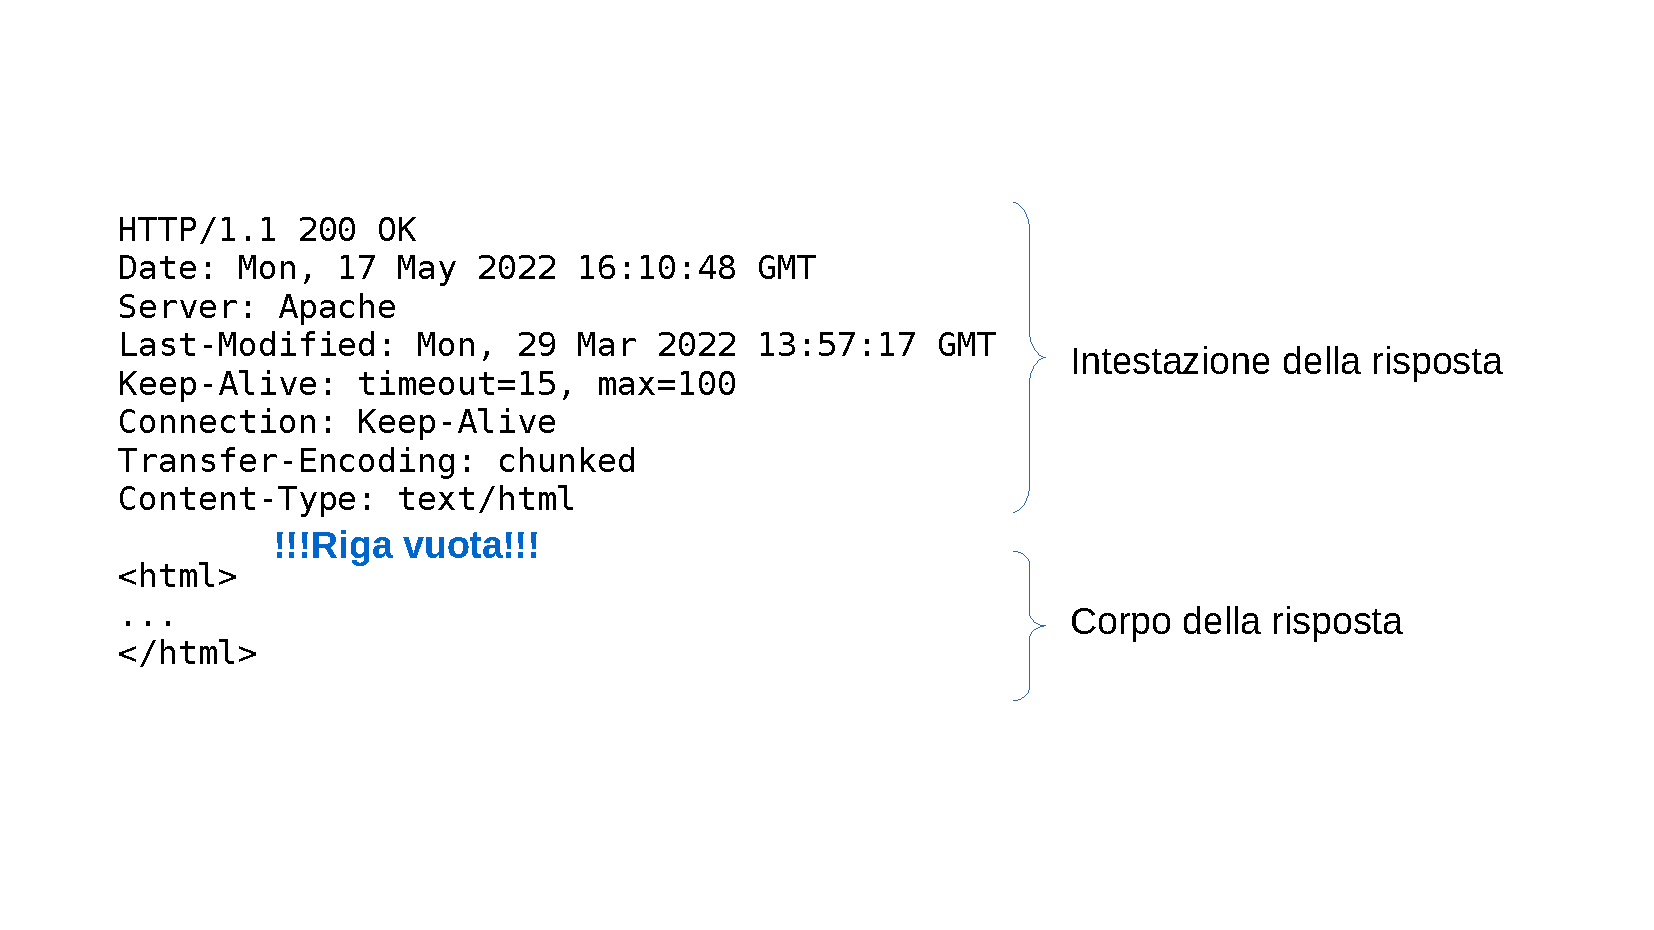
\includegraphics[width=\textwidth]{img/risposta_http.pdf}
		\caption{Messaggio di risposta.}
	\end{figure}\newpage

	\subsection{Hyper Text Markup Language (HTML) e Cascading Style Sheets (CSS)}
	
	\textcolor{Red3}{\textbf{HTML}} è un linguaggio testuale di descrizione di una pagina, in particolare è la specializzazione del generico XML (\emph{eXtensible Markup Language}). HTML si basa sui \dquotes{tag} annidati, i quali eventualmente contengono attributi.\newline
	
	\noindent
	Questo linguaggio, spesso viene utilizzato con un altro linguaggio chiamato \textbf{CSS}.\newline
	
	\noindent
	\textcolor{Green4}{\textbf{Esempi}} di codice HTML:
	\lstinputlisting[language=HTML]{code/css.html}
	E CSS:
	\lstinputlisting{code/styles.css}
	
	\longline
	
	\subsubsection{HTML: tag per richiamare immagini}
	
	Viene utilizzato \dquotes{\textsf{img src}} per richiamare le immagini:
	\lstinputlisting[language=HTML]{code/immagini.html}\newpage
	
	\subsubsection{HTML: tag per il collegamento ipertestuale}
	
	Viene utilizzato \dquotes{\textsf{href}} per il collegamento ipertestuale:
	\lstinputlisting[language=HTML]{code/link.html}
	
	\longline
	
	\subsubsection{Document Object Model (DOM)}
	
	Il \textcolor{Red3}{\textbf{Document Object Model (DOM)}} è una forma di rappresentazione dei documenti (pagina) strutturati come modello orientato agli oggetti.
	
	\longline
	
	\subsection{Javascript}
	
	\textcolor{Red3}{\textbf{Javascript}} è un linguaggio di programmazione multi paradigma orientato agli eventi, utilizzato sia nella programmazione lato client web che lato server. È facile trovarlo all'interno di codice HTML anche grazie al suo tag riconoscibile: \textsf{<script>}.
	
	Tuttavia, è difficile trovare del codice Javascript pure scritto nelle pagine HTML. Solitamente vengono create vere e proprie librerie così da rendere il codice più leggibile e mantenibile.\newline
	
	\noindent
	Un \textcolor{Green4}{\textbf{esempio}} di codice Javascript:
	\lstinputlisting[language=HTML]{code/javascript.html}\newpage
	
	\noindent
	Javascript trova il suo grande utilizzo con gli \textbf{eventi causati dall'utente}, per esempio con la pressione di un bottone all'interno di una pagina web:
	\lstinputlisting[language=HTML]{code/javascript-evento.html}
	
	\longline
	
	\subsubsection{Javascript e Document Object Model (DOM)}
	
	Il \textbf{\emph{Document Object Model} consente di trasformare una pagina web da documento statico a \emph{Graphical User Interface} (GUI)}, cioè interattivo.
	
	Infatti, grazie al codice Javascript contenuto nella pagina HTML ed eseguito dal browser, l'utente può modificare lo stato della pagina web a seconda di determinate azioni. Quindi, la pagina web si automodifica e assume le sembianze di una applicazione web, chiamata in gergo \emph{web application}.\newline
	
	\noindent
	Alcuni \textcolor{Green4}{\textbf{esempi}} di codice interattivo:
	\begin{itemize}
		\item Per avere un riquadro con la pagina web ANSA:
		\lstinputlisting[language=HTML]{code/javascript-load.html}\newpage
		
		\item Per avere un timer che alla fine del tempo stampa \dquotes{Hello}:
		\lstinputlisting[language=HTML]{code/javascript-timer.html}
		
		\item Per avere lo stesso effetto del punto precedente ma utilizzando una \textbf{funzione}:
		\lstinputlisting[language=HTML]{code/javascript-timer2.html}
	\end{itemize}\newpage
	
	\subsection{Uniform Resource Locator (URL)}
	
	Chiamato anche Universal Resource Locator, l'\textcolor{Red3}{\textbf{URL}} consente di identificare in maniera univoca una risorsa HTTP in qualsiasi parte della rete mondiale.\newline
	
	\noindent
	È \textbf{strutturato} in tre parti:
	\begin{itemize}
		\item Il protocollo utilizzato a livello di applicazione, di trasporto e la porta utilizzata, per esempio HTTP con protocollo TCP e porta 80;
		
		\item Nome/IP dell'host che eroga tale risorsa;
		
		\item Nome della risorsa con il percorso logico completo.
	\end{itemize}\newpage
	
	\subsection{Passare dei dati al server web col metodo GET}
	
	Il codice HTML per utilizzare il metodo GET è il seguente:
	\lstinputlisting[language=HTML]{code/form-get.html}
	La pagina web visualizzata è la seguente:
	\begin{figure}[!htp]
		\centering
		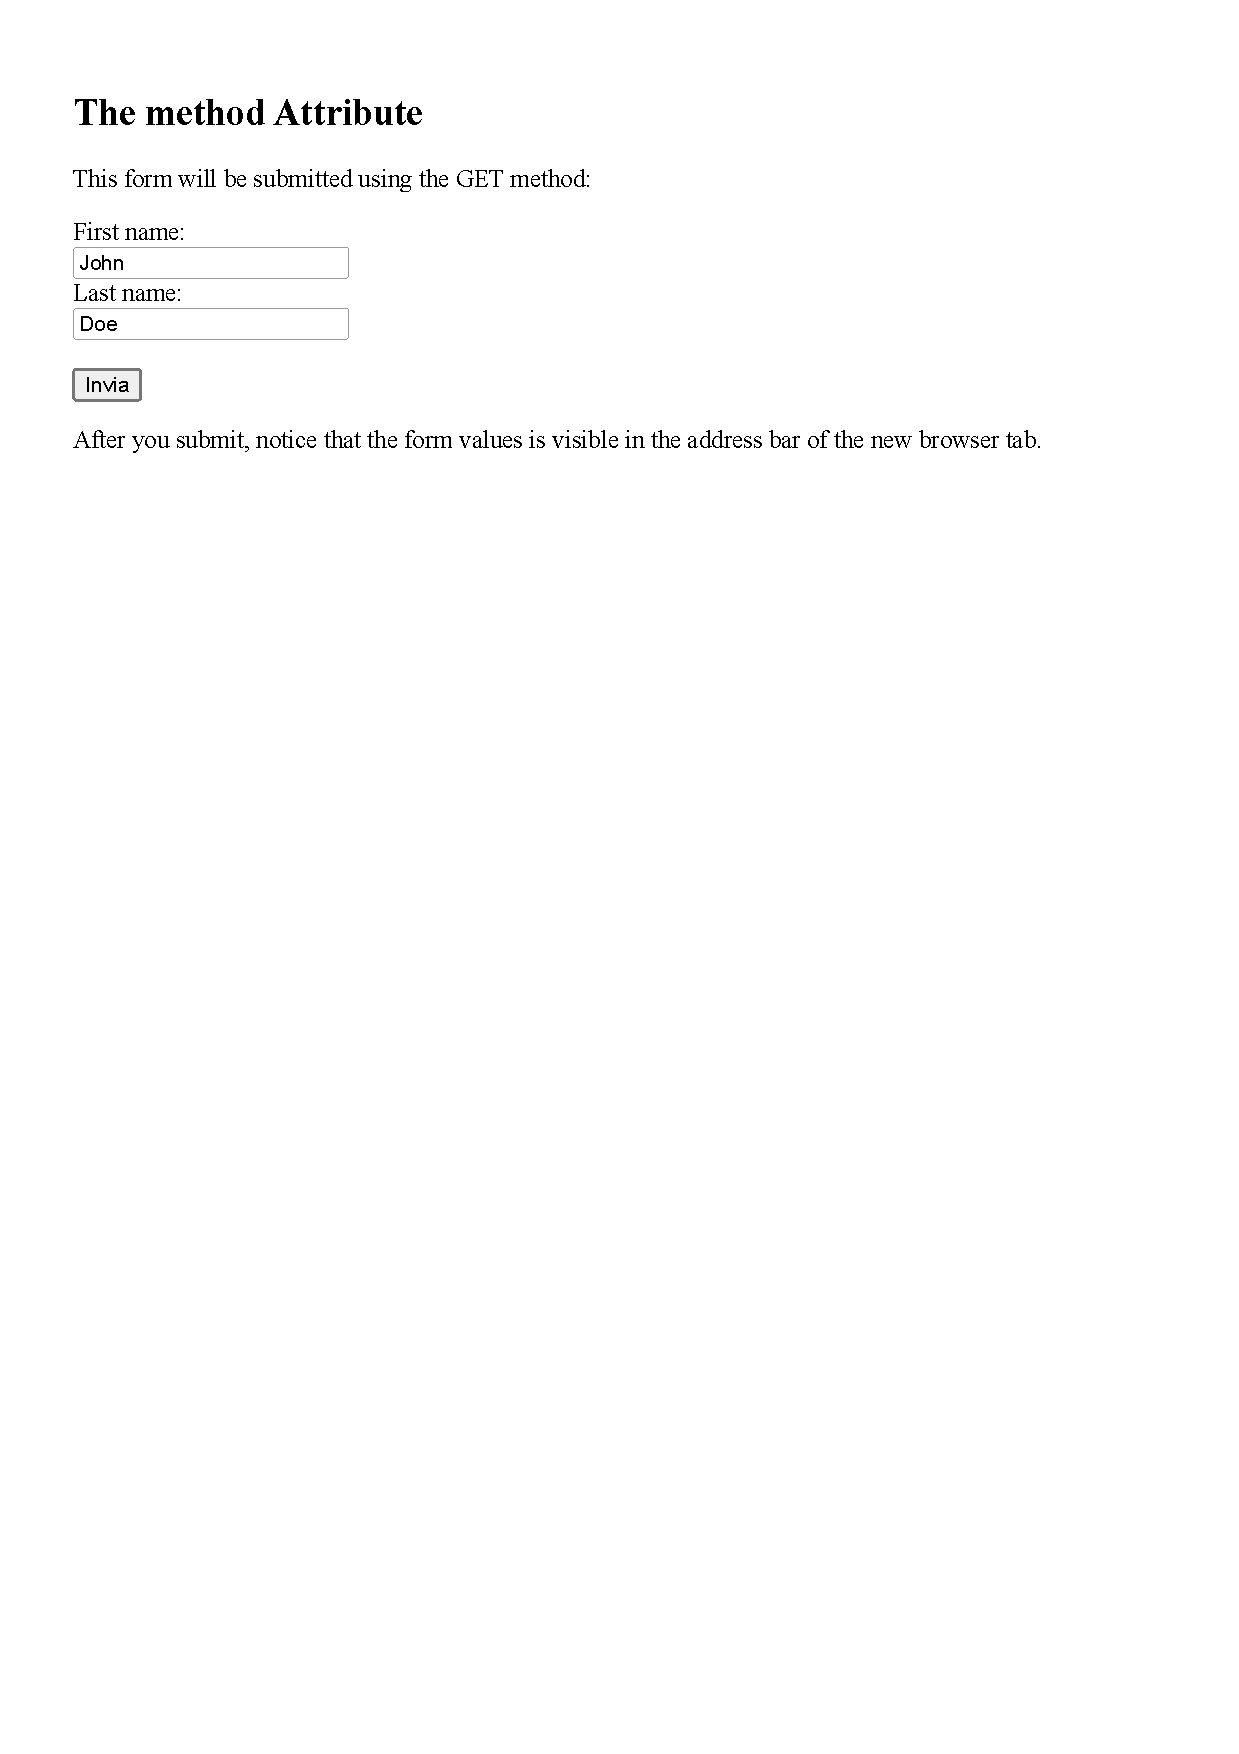
\includegraphics[width=\textwidth]{img/form-get.pdf}
	\end{figure}
	
	\noindent
	Una volta inserito nome e cognome, alla pressione del tasto, i dati saranno inviati al \emph{localhost} aggiungendo come parametri nell'URL \textsf{fname=name} e \textsf{lname=name}, dove al posto di name vengono inseriti nome e cognome. Il link risulta: \url{http://127.0.0.1/action?fname=John&lname=Doe}.\newpage
	
	\begin{figure}[!htp]
		\centering
		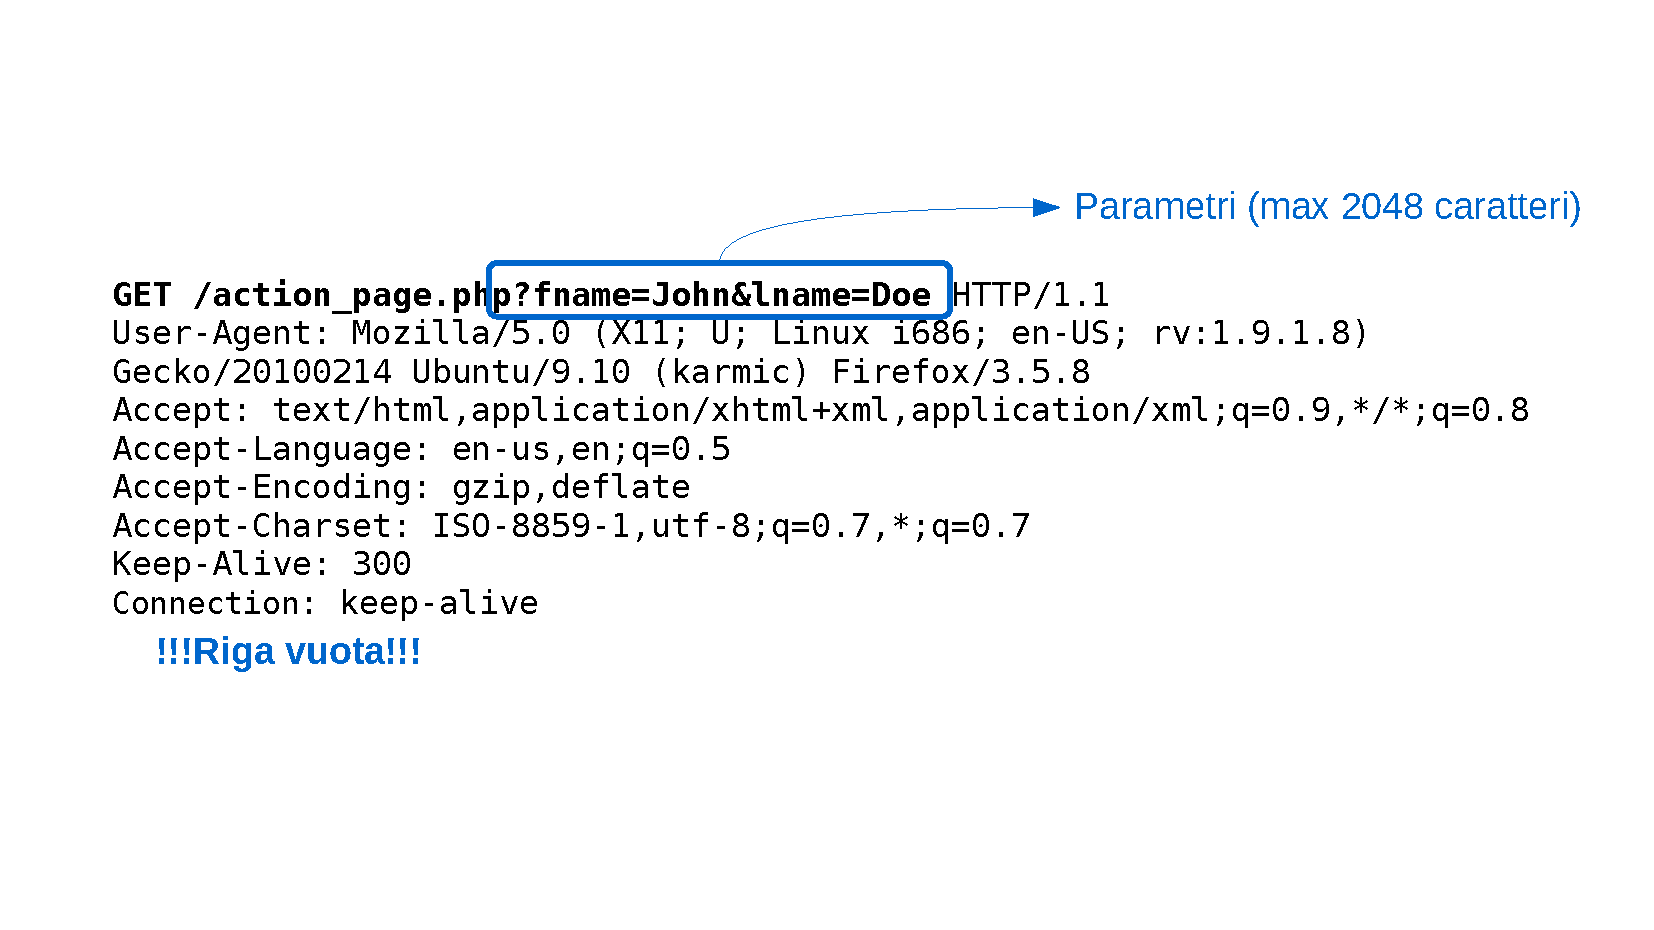
\includegraphics[width=\textwidth]{img/richiesta_get.pdf}
		\caption{La richiesta GET HTTP.}
	\end{figure}\newpage

	\subsection{Passare dei dati al server web col metodo POST}
	
	Il codice HTML per utilizzare il metodo POST è il seguente:
	\lstinputlisting[language=HTML]{code/form-post.html}
	La pagina web visualizzata è la seguente:
	\begin{figure}[!htp]
		\centering
		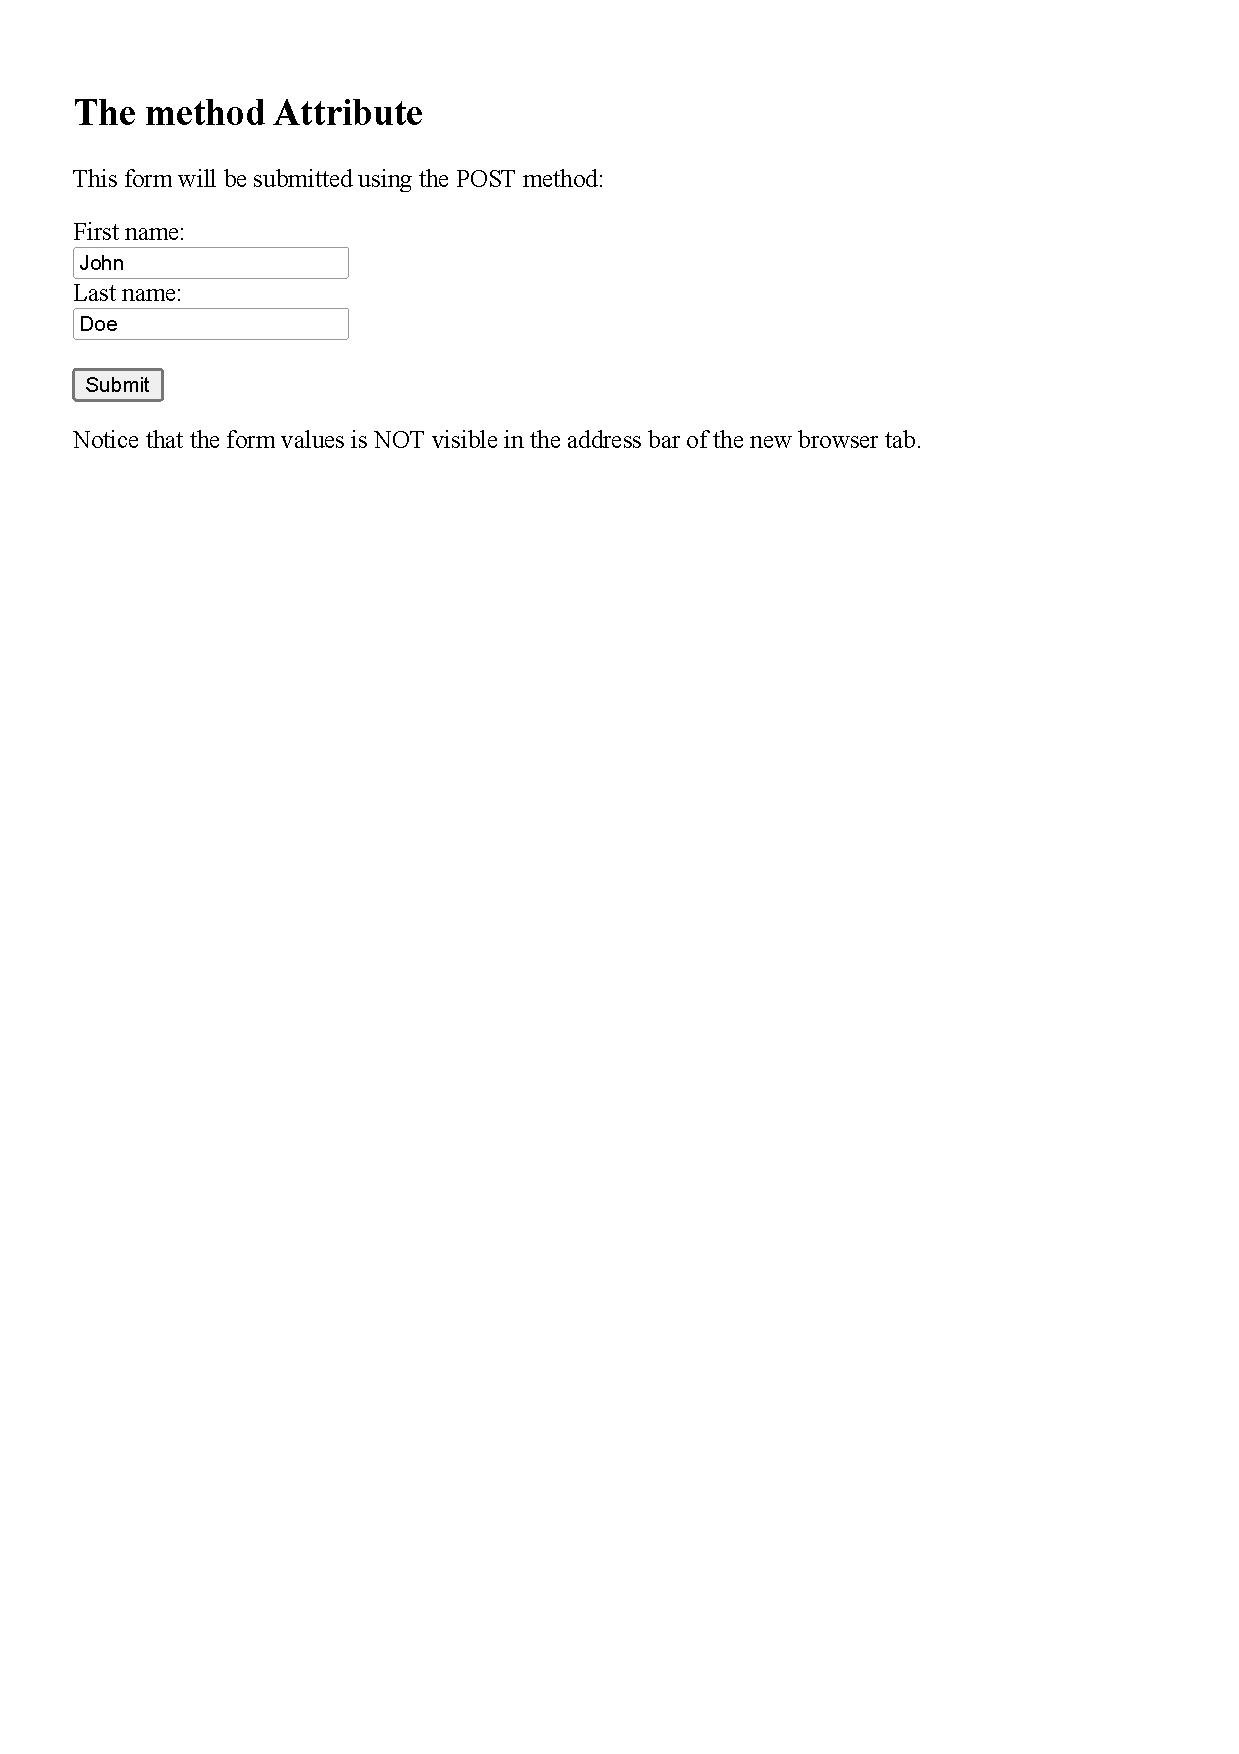
\includegraphics[width=\textwidth]{img/form-post.pdf}
	\end{figure}
	
	\noindent
	Una volta inserito nome e cognome, alla pressione del tasto, i dati saranno inviati al \emph{localhost}. \textbf{A differenza del metodo GET}, i parametri non vengono specificati nell'URL, di conseguenza la sicurezza aumenta. Il link dunque risulta: \url{http://127.0.0.1/action}.\newline
	
	\noindent
	I valori vengono inseriti all'interno della richiesta HTTP.\newpage
	
	\begin{figure}[!htp]
		\centering
		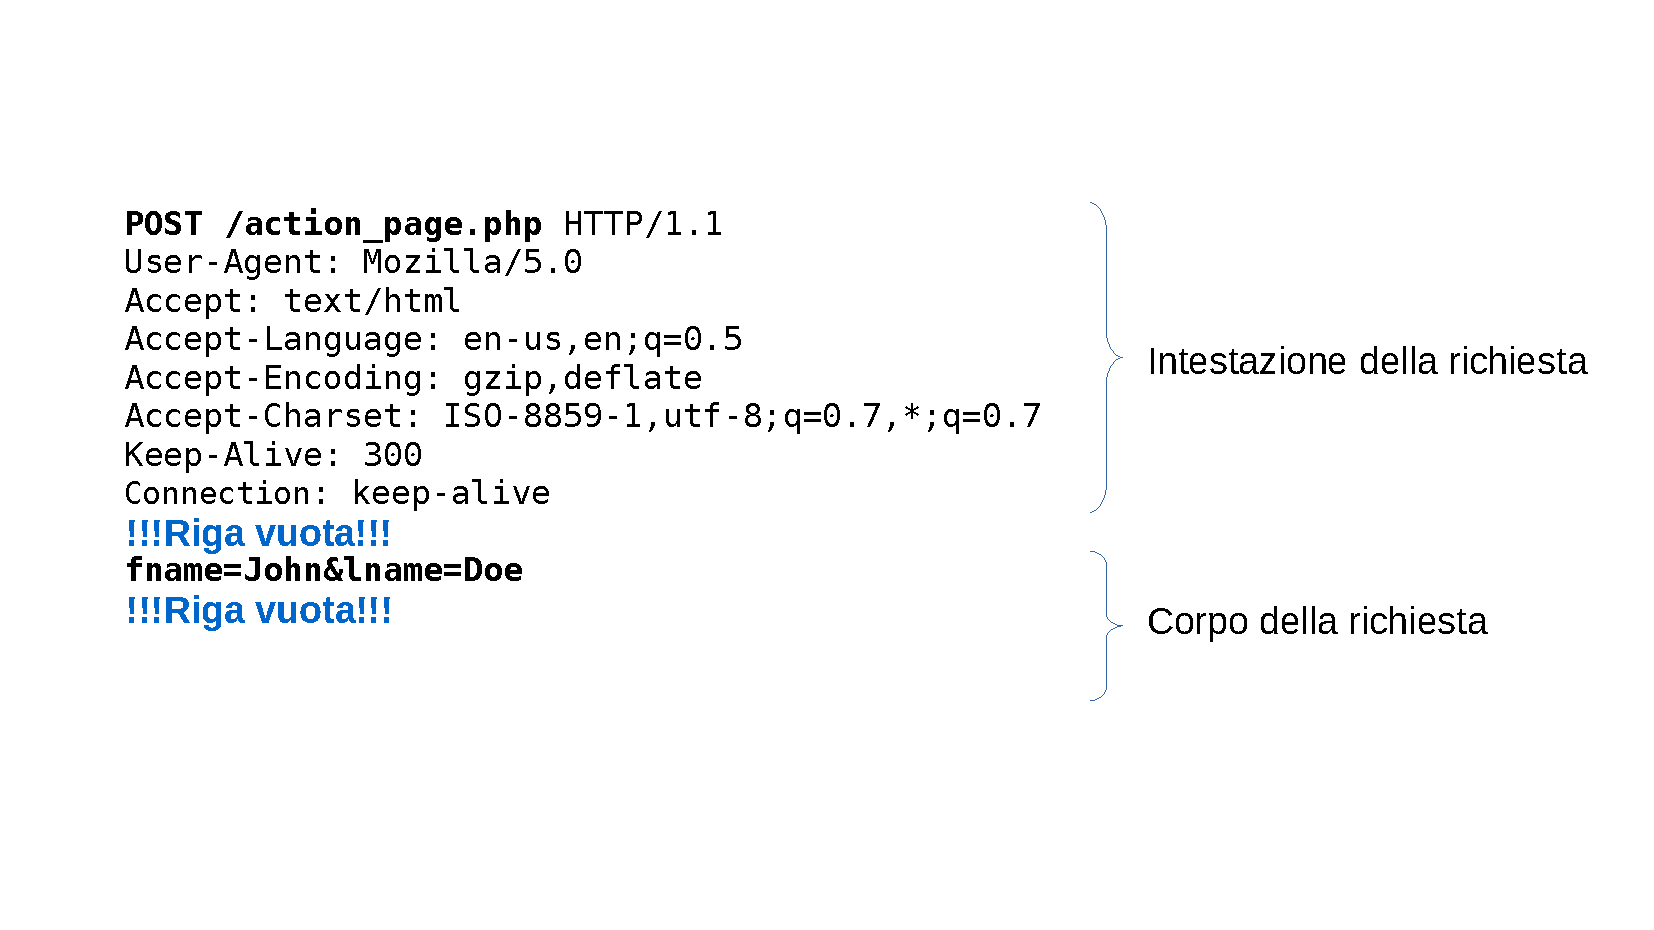
\includegraphics[width=\textwidth]{img/richiesta_post.pdf}
		\caption{La richiesta POST HTTP.}
	\end{figure}\newpage

	\subsection{Common Gateway Interface (CGI)}
	
	Il \textcolor{Red3}{\textbf{Common Gateway Interface (CGI)}} è una tecnologia utilizzata dai \emph{web server} per interfacciarsi con applicazioni esterne generando contenuti web dinamici.\newline
	
	\noindent
	Ogni qualvolta che un \emph{client} richiede al web server un URL corrispondente a un documento HTML, gi viene restituito un documento statico. Al contrario, se l'URL corrisponde a un programma CGI, il server lo esegue in tempo reale, generando dinamicamente informazioni per l'utente. Sostanzialmente è l'\textbf{esecuzione di un determinato programma sul server}.
	
	Di conseguenza, il browser diventa il \emph{client} di molte applicazioni di rete, per esempio la posta elettronica.
	
	\begin{figure}[!htp]
		\centering
		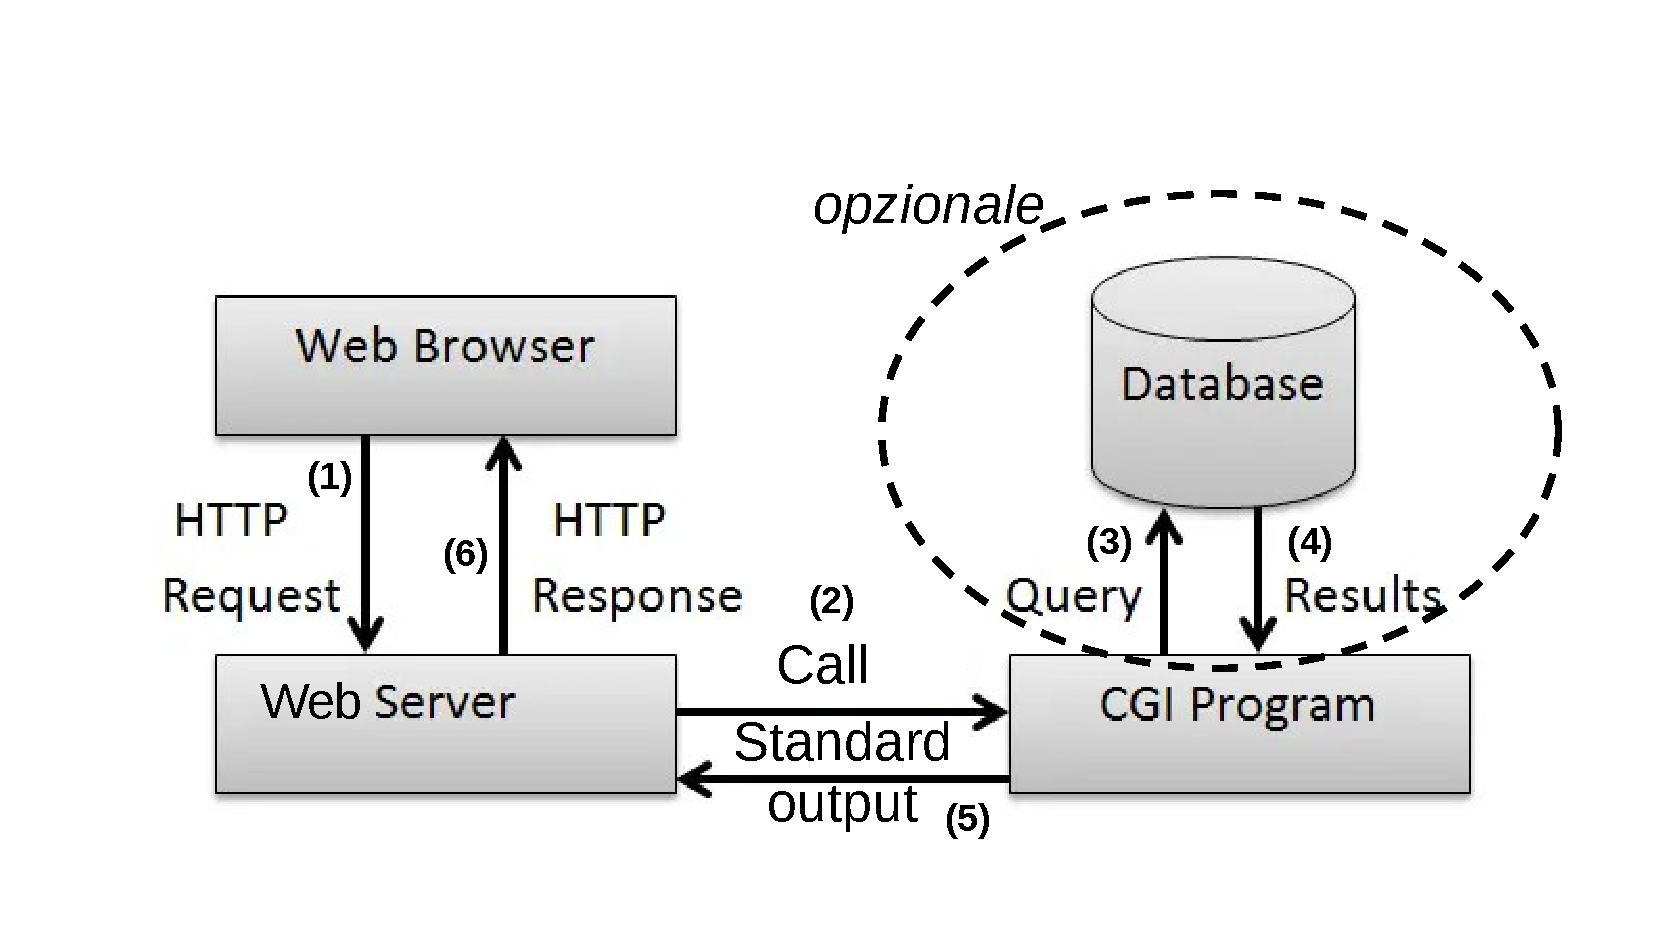
\includegraphics[width=\textwidth]{img/CGI.pdf}
		\caption{Fasi del CGI.}
	\end{figure}

	\noindent
	Degli \textcolor{Green4}{\textbf{esempi}} di esecuzione lato server di un programma sono un eseguibile come il client della posta elettronica, oppure un codice PHP, Java, NodeJS, ecc.\newpage
	
	\begin{figure}[!htp]
		\centering
		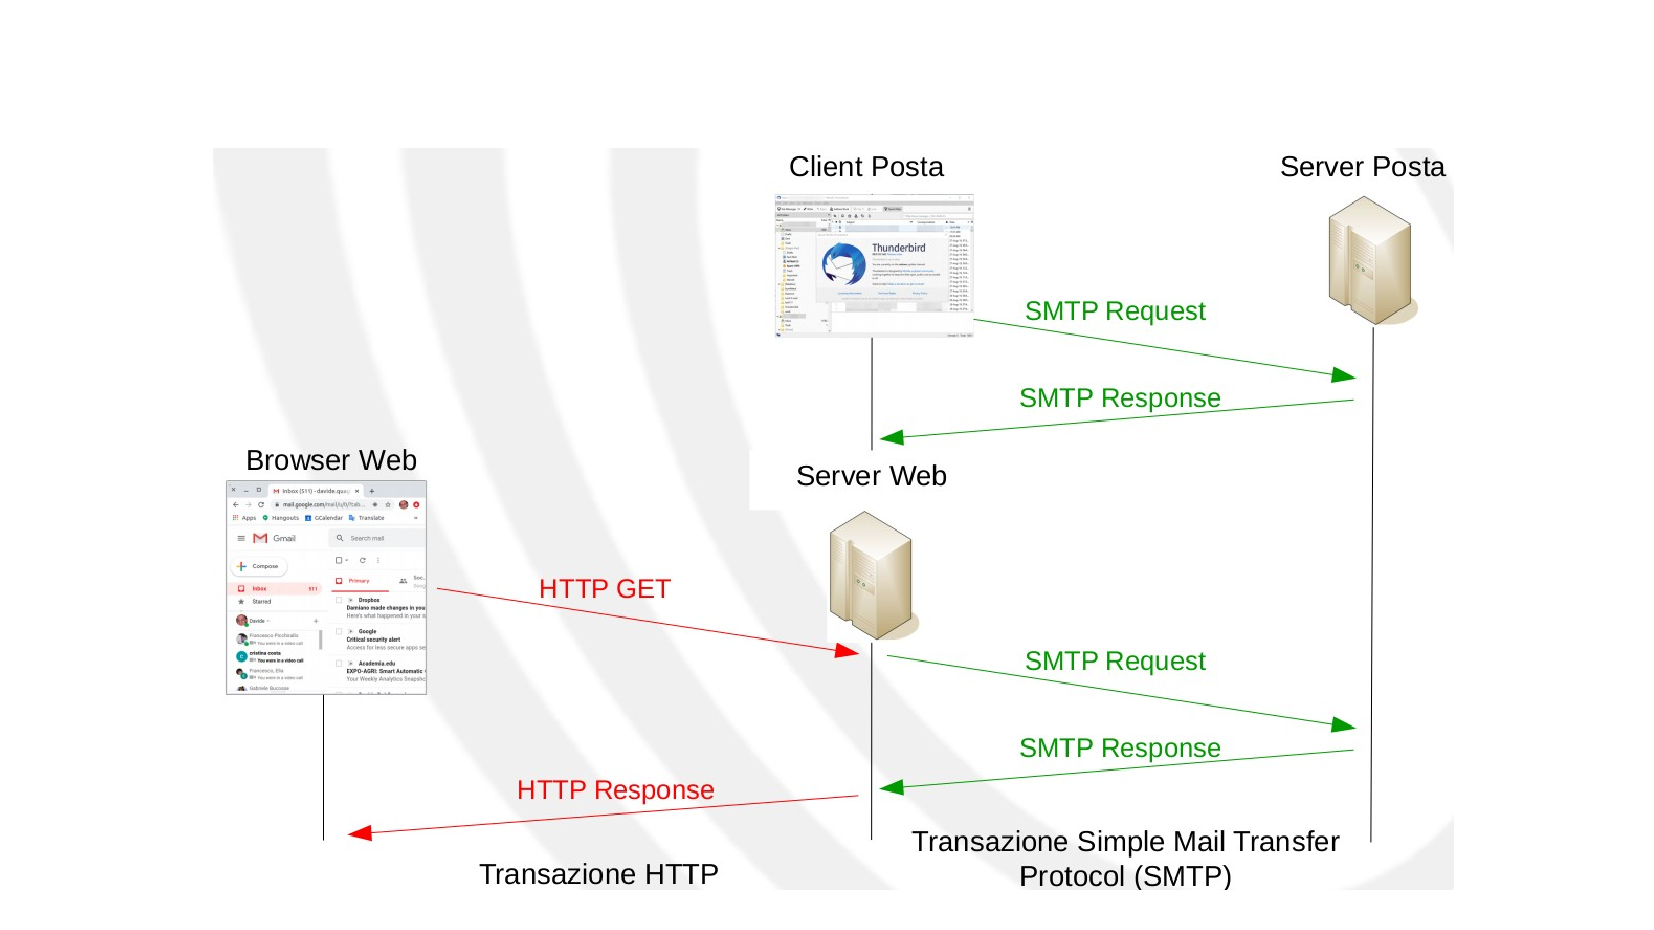
\includegraphics[width=\textwidth]{img/CGI_esempio.pdf}
		\caption{Esempio di CGI, la classica posta elettronica.}
	\end{figure}\newpage

	\subsection{Web socket}
	
	La \textcolor{Red3}{\textbf{web socket}} è una tecnologia web che fornisce canali di comunicazione chiamati \emph{full-duplex}, cioè bidirezionali, attraverso una singola connessione TCP. Viene utilizzato principalmente per realizzare applicazioni che forniscono contenuti e giochi in tempo reale. Questo perché \textbf{il protocollo consente maggiore interazione tra browser e server} grazie al alcune caratteristiche.\newline
	
	\noindent
	Innanzitutto è un \textbf{protocollo a livello di applicazione}, per cui è un \textbf{metodo alternativo a HTTP e HTTPS}. Ha la caratteristica fondamentale di \textbf{comunicazione simmetrica} tra \emph{browser} e \emph{web server}, ovverosia che \textbf{i processi possono \dquotes{prendere l'iniziativa} e inviare dei dati alla controparte}. Inoltre, nasce da una sessione HTTP/HTTPS attraverso un'operazione chiamata \textbf{Protocol Upgrade}.
	\begin{figure}[!htp]
		\centering
		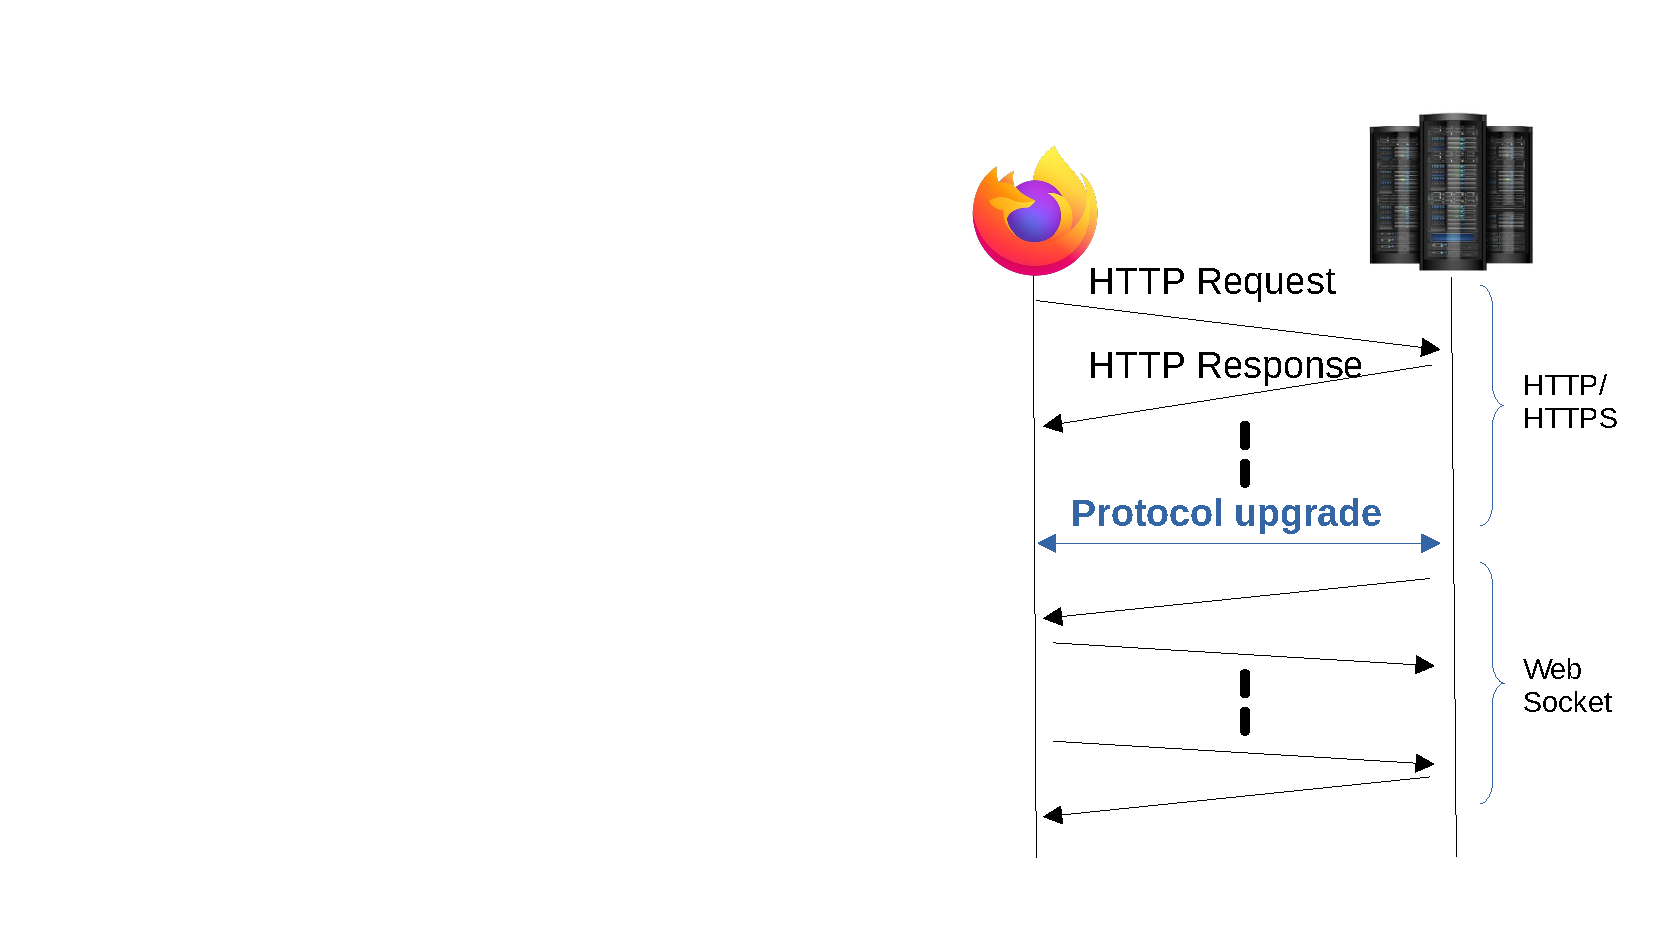
\includegraphics[width=.5\textwidth]{img/web_socket.pdf}
		\caption{Esempio di web socket e Protocol Upgrade.}
	\end{figure}
	
	\noindent
	Nel messaggio HTTP, ci sono due campi che vengono modificati per indicare il Protocol Upgrade: \textsf{Upgrade} e \textsf{Connection}. Entrambi i campi vengono modificati con i rispettivi valori \textsf{websocket} e \textsf{Upgrade}.\newpage
	
	\noindent
	\begin{figure}[!htp]
		\centering
		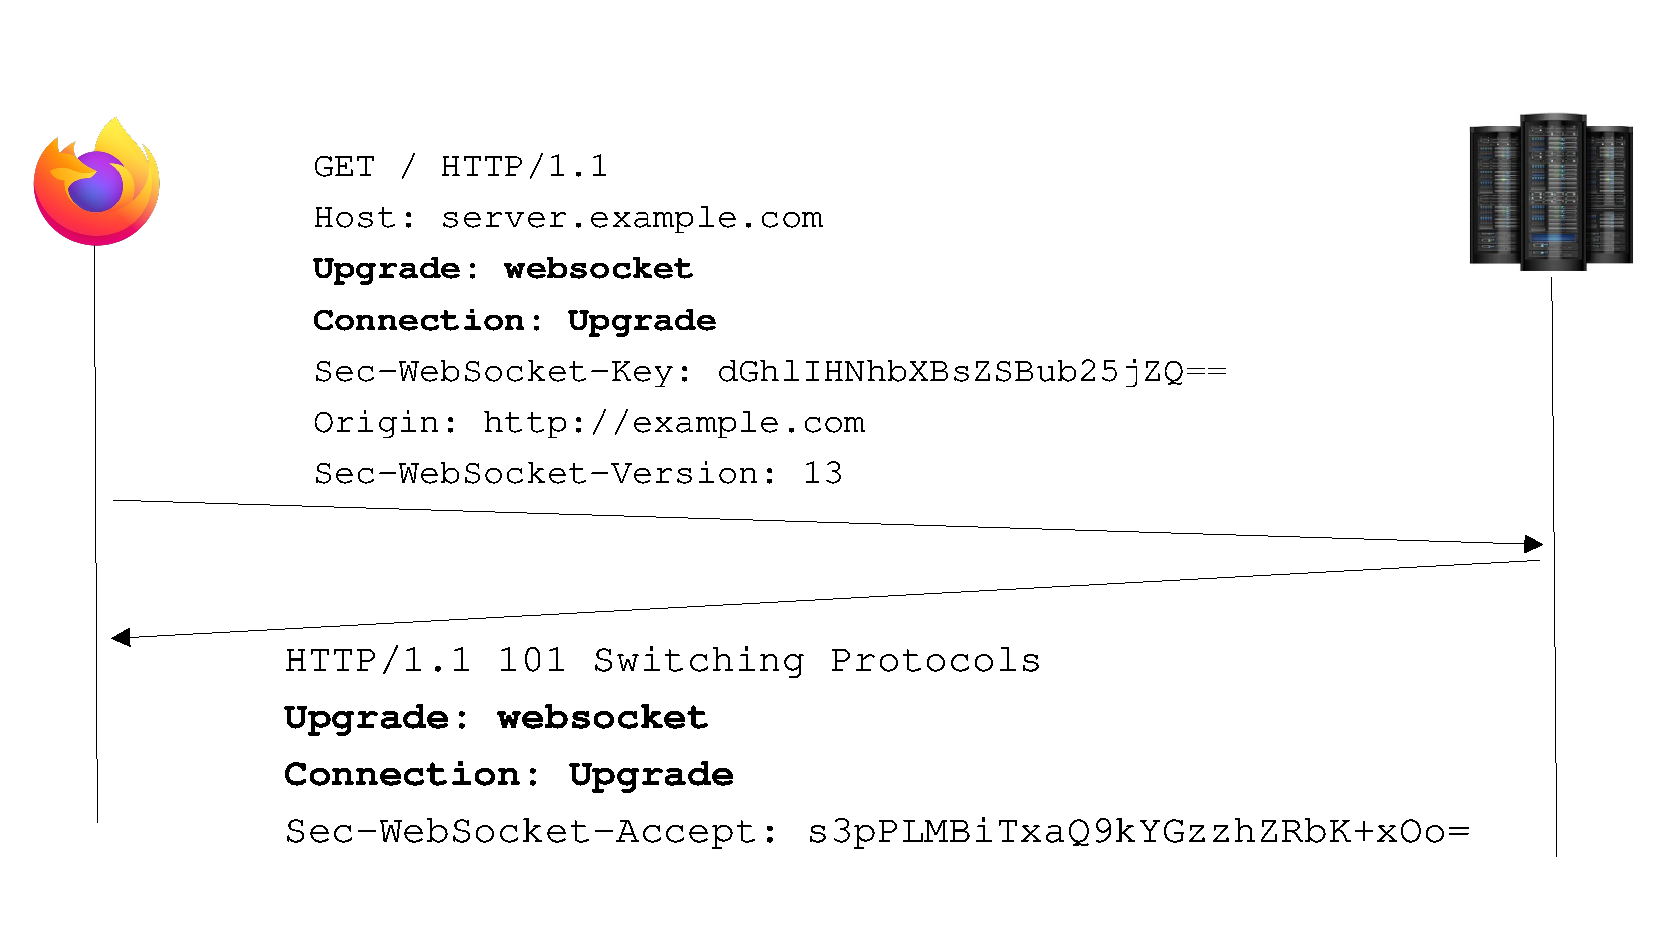
\includegraphics[width=\textwidth]{img/protocol_upgrade.pdf}
		\caption{Il Protocol Upgrade nel dettaglio.}
	\end{figure}\newpage

	\subsubsection{Approfondimento WebSocket}
	
	Il \textbf{WebSocket} è un protocollo di comunicazione web che fornisce un canale di \textbf{comunicazione bidirezionale} attraverso una singola connessione TCP inizialmente utilizzata per il protocollo HTTP.
	
	Il protocollo consente \textbf{maggiore interazione tra browser e server}, facilitando inoltre la realizzazione di applicazioni web che devono fornire contenuti in tempo reale. Tutto questo è possibile poiché i \textbf{WebSocket concedono al server di \dquotes{prendere l'iniziativa} ed effettuare dei \emph{push} autonomi di dati verso il browser per aggiornarlo}. Ovviamente questo non è possibile con il classico protocollo HTTP. Per \textbf{\emph{comunicazione bidirezionale}} si intende una comunicazione in entrambe le direzioni \underline{simultaneamente}.\newline
	
	\noindent
	I WebSocket sono basati sul protocollo TCP e nascono da una connessione HTTP grazie ad un \textbf{Upgrade Request} richiesto dal client al server. Il browser comunica questa richiesta speciale al server tramite alcune voci nell'intestazione del messaggio. Inoltre, il WebSocket consente connessioni per un lungo periodo.\newline
	
	\noindent
	In sintesi, le \textbf{\underline{caratteristiche}} di questo protocollo:
	\begin{itemize}
		\item Si \textbf{basa sul protocollo TCP}, la quale inizialmente utilizza il protocollo HTTP, ma grazie alla richiesta speciale Upgrade Request, essa muta nel protocollo WebSocket;
		
		\item \textbf{Connessione bidirezionale} (\emph{full-duplex}), quindi aumento della facilità nella realizzazione di applicazioni web che forniscono contenuti in tempo reale;
		
		\item \textbf{Utilizzo di porte note} (\emph{Well-know ports}), in particolare quelle dedicate al protocollo HTTP, quindi la 80 e la 443;
		
		\item \textbf{Connessioni per un lungo periodo}.
	\end{itemize}

	\longline
	
	\subsubsection{Limitazioni}
	
	Nonostante la grande utilità che apporta il protocollo WebSocket, esso non è la soluzione a tutto. Infatti, \textbf{HTTP ha ancora un ruolo chiave nella comunicazione client-server} per vari motivi:
	\begin{itemize}
		\item \textbf{Invio e chiusura delle connessioni per trasferimenti di dati di tipo one-time}, come i caricamenti iniziali. Il protocollo HTTP è più efficiente del WebSocket;
		
		\item \textbf{Utilizzo più intelligente} da parte di HTTP delle \textbf{risorse} grazie alla chiusura delle connessioni una volta terminate le operazioni. Al contrario, il WebSocket mantiene una connessione attiva più a lungo rischiando di sprecare risorse inutilmente;
		
		\item \textbf{WebSocket riservato solo agli utenti con JavaScript abilitato} e quindi a coloro che posseggono browser moderni a discapito, per esempio, dei sistemi \emph{embedded}.
	\end{itemize}\newpage

	\subsection{WebSocket-Chat}
	
	WebSocket-Chat è un progetto \dquotes{giocattolo} \textbf{realizzato per comprendere al meglio la tecnologia offerta dal protocollo WebSocket}. Esso utilizza vari linguaggi di programmazione: JavaScript, Node.js (\href{https://it.wikipedia.org/wiki/Node.js}{framework per realizzare applicazioni Web in JavaScript}), HTML, CSS e una parte aggiuntiva chiamata Console con Ispezione Network (monitoraggio da parte del browser con scambio tra i pacchetti).
	
	\longline
	
	\subsubsection{Node.js e l'approccio asincrono}
	
	Il framework \textcolor{Red3}{\textbf{Node.js}} (\href{https://it.wikipedia.org/wiki/Node.js}{Wikipedia}, \href{https://nodejs.org/it}{sito ufficiale Node.js}) è nato per realizzare applicazioni Web in JavaScript. Solitamente viene utilizzato lato client (\emph{client-side}) per realizzare applicazioni tipicamente lato server (\emph{server-side}).\newline
	
	\noindent
	La \textbf{caratteristica principale} di Node.js è la possibilità di accedere alle risorse del sistema operativo in modalità \emph{event-driven} (\href{https://it.wikipedia.org/wiki/Programmazione_a_eventi}{programmazione orientata agli eventi}) e \underline{non} sfruttando il classico modello basato su processi/thread concorrenti, utilizzato dai classici web server.\newline
	
	\noindent
	Il modello \textbf{\emph{event-driven}}, tradotto in programmazione orientata agli eventi, si basa sulla \textbf{mutazione di stato nel momento in cui si manifesta un evento}.
	
	A differenza della programmazione procedurale (\emph{C-style}) in cui ogni azione viene eseguita una dopo l'altra con un determinato ordine, nella programmazione ad eventi le azioni sono asincrone e seguono un ordine dettato dalla manifestazione degli eventi.\newline
	
	\noindent
	L'\textbf{approccio asincrono} comporta una \textcolor{Green4}{\textbf{grande efficienza}} soprattutto in ambito di \emph{networking} poiché capita spesso di effettuare richieste e di rimanere in attesa di un'eventuale risposta. Grazie all'approccio asincrono, \textbf{durante l'attesa possibile effettuare altre operazioni che non dipendono dalla richiesta effettuata}.
	
	\longline
	
	\subsubsection{Descrizione dell'applicazione}
	
	Il progetto mira ad avere una chat multiutente a cui collegarsi tramite browser. Le \emph{features} implementate sono le seguenti:
	\begin{itemize}
		\item Registrazione del nome di contatto che si vuole avere quando si accede alla chat.
		
		\item Invio dei messaggi in broadcast a tutti gli utenti attualmente collegati alla chat.
	
		\item Visualizzazione dei messaggi inviati col nome della persona che lo ha inviato.
	\end{itemize}\newpage

	\subsubsection{Codice Back-end server}\label{codice Back-end server}
	
	\lstinputlisting[language=JavaScript]{code/server.js}
	
	\begin{itemize}
		\item (3) \textcolor{Red3}{\textbf{Express.js}} è una libreria di Node.js che consente di costruire applicazioni web molto facilmente (\href{https://en.wikipedia.org/wiki/Express.js}{Wikipedia}, \href{https://expressjs.com/}{sito ufficiale}). L'unica cosa importante da sapere è che la prima linea di codice crea una variabile \textsf{express}, che necessita della relativa libreria Express.js, e viene \textbf{utilizzata per creare il server web in ascolto sulla porta 4000}.
		
		\item (4) \textcolor{Red3}{\textbf{Socket.IO}} è una libreria JavaScript \textbf{utilizzata per implementare il protocollo WebSocket} e racchiude molte \textbf{funzioni} tra le quali:
		\begin{itemize}
			\item \textbf{Broadcasting} a tutti i socket collegati;
			
			\item \textbf{Salvataggio} dei dati riguardanti ciascun utente;
			
			\item Approccio \textbf{asincrono di I/O}.
		\end{itemize}
	
		\item (6-13) Alla riga 7 viene effettuato il vero e proprio \emph{import} della libreria e viene creato il socket;
		
		Alla riga 11 il server si mette in ascolto, sulla porta 4000, e (riga 12) stampa sul terminale la stringa \dquotes{waiting for HTTP requests on port 4000,}.
		
		
		\item (21) Una volta ricevuta una connessione da parte di un client, il server ricerca all'interno della cartella chiamata \textsf{public}, il relativo file \dquotes{.html} da inviare al mittente.
		
		\item (29) Alla conferma di connessione instaurata e di file ricevuto, il server prende l'iniziativa ed esegue un \textbf{Upgrade Request} trasformando la connessione in una WebSocket.
		
		\item (30-38) Il server rimane in attesa, in particolare questo accade alla linea 35. Nel momento in cui un client scatena un evento, ovvero invia un messaggio con il tag \textsf{message}, il server lo inoltrerà a tutti i client connessi mediante l'oggetto \textsf{sockets}.
	\end{itemize}

	\longline
	
	\subsubsection{Codice Front-end HTML}
	
	\lstinputlisting[language=HTML]{code/index.html}
	Il codice HTML consente di far visualizzare l'interfaccia utente creata da JavaScript. In particolare, nella pagina è possibile leggere e inviare messaggi.\newline
	
	\noindent
	L'unica osservazione da fare è il tag \textsf{<script>}, il quale contiene il link del file .js da eseguire all'apertura del file HTML (paragrafo~\ref{codice Front-end JavaScript}). Ovviamente si intende il codice a riga 21, ovvero quello necessario per la chat.\newpage
	
	\subsubsection{Codice Front-end JavaScript}\label{codice Front-end JavaScript}
	
	\lstinputlisting[language=JavaScript]{code/chat.js}
	\begin{itemize}
		\item (3-6) Finché non viene inserito un nome, il codice continua a chiederlo.
		
		\item (9-13) Vengono inizializzate le variabili che acquisiscono i tag presenti nella pagina HTML.
		
		\item (15-16) Viene scritto il nome dell'utente nella pagina web e impostato il valore.
		
		\item (19) Viene creato il socket che deve connettersi al server.
		
		\item (22-30) Sul bottone di invio del messaggio, viene aggiunto un nuovo evento JavaScript. Quest'ultimo si attiverà nel momento in cui l'utente cliccherà sul bottone. Una volta premuto, se il messaggio non sarà vuoto, verrà inviato al server (con tag \textsf{message}!) il messaggio (riga 25) e il nome dell'utente (riga 26). Una volta inviato, viene svuotato il valore del messaggio.
		
		\item (32-35) Sono la stampa del messaggio ricevuto. Si noti il segno \dquotes{+=} che indica che i vari messaggi ricevuti vengono concatenati.
	\end{itemize}\newpage

	\subsubsection{Esecuzione del Front-end e del Back-end}
	
	Il server web utilizzato è Node.js che consente di eseguire codice JavaScript \emph{server-side} per creare il Back-end. Invece, il Front-end è realizzato mediante codice JavaScript eseguito dentro il browser.\newline
	
	\noindent
	Passaggi da eseguire su Windows:
	\begin{enumerate}
		\item Download del file di installazione dal sito ufficiale: \url{https://nodejs.org/it/download}
		
		\item Eseguire il Back-end:
		\begin{enumerate}
			\item Scaricare lo zip fornito su Moodle con nome \dquotes{WebSocket\_Chat};
			\item Aprire un terminale e posizionarsi nella cartella contente il file \textsf{server.js};
			\item Eseguire il comando: \textsf{node.exe server.js}.
		\end{enumerate}
		
		\item Eseguire il Front-end:
		\begin{enumerate}
			\item Aprire il browser alla pagina: \url{http://localhost:4000};
			\item (Opzionale) Aprire più finestre del browser così da simulare l'accesso da parte di più utenti.
		\end{enumerate}
	\end{enumerate}\newpage
	
	\subsubsection[\textcolor{Red3}{\textbf{Esercizi}}]{Esercizi}
	
	\noindent	
	\textcolor{Red3}{\textbf{\emph{\underline{Esercizio 1}}}}\newline
	
	\noindent
	Lanciare l'applicazione dopo aver fatto partire l'ispezione del Network tramite la console di sviluppo del browser. Ogni quanto tempo il client fa sapere al server che è ancora connesso? È un'azione dovuta all'implementazione della chat o insita nel WebSocket? A cosa sere tale procedura?\newline
	Lanciare Wireshark e vedere cosa passa in rete sulla connessione TCP interessata.\newline
	
	\noindent	
	\textcolor{Green4}{\textbf{\emph{\underline{Soluzione esercizio 1}}}}\newline
	
	\noindent
	Per analizzare la rete si utilizza il software Wireshark che consente di analizzare il flusso di pacchetti in entrata e in uscita. All'apertura del software, andando nella sezione \dquotes{\emph{Adapter for loopback traffic capture}} sarà possibile seguire tutti i pacchetti che riguardano il localhost. Per filtrare il risultato dei pacchetti, si inserisce la stringa \dquotes{websocket} nella barra in alto, così da mostrare solamente quei pacchetti con protocollo WebSocket:
	\begin{figure}[!htp]
		\centering
		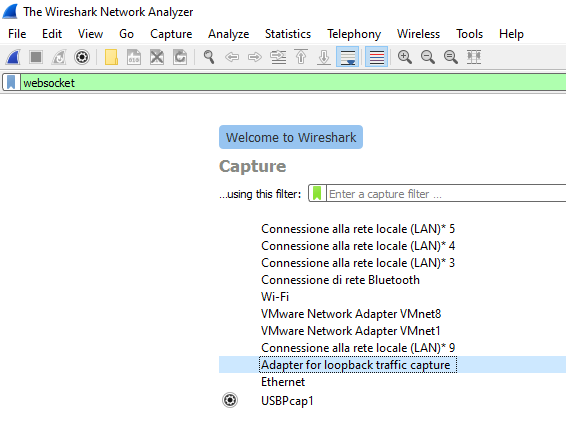
\includegraphics[width=\textwidth]{img/soluzioni_websocket-chat/wireshark-1.png}
	\end{figure}

	\noindent
	A questo punto, si aprono tre, quattro client. Quindi, si scrive l'URL localhost:4000 nel browser. Dato che il server non è in esecuzione, il browser non riesce a collegarsi al localhost:4000 poiché vede tale porta inutilizzata. Di conseguenza, il traffico catturato da Wireshark è inesistente.\newline

	\noindent
	Avviando il server, in automatico vedrà il collegamento dei 3/4 client avviati precedentemente. Di conseguenza, su Wireshark appariranno dei pacchetti corrispondenti al collegamento dei client al server:
	\begin{figure}[!htp]
		\centering
		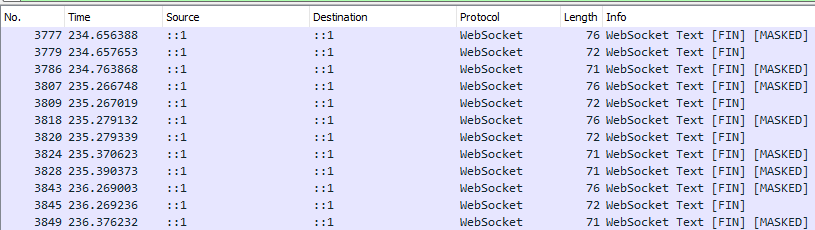
\includegraphics[width=\textwidth]{img/soluzioni_websocket-chat/wireshark-2.png}
	\end{figure}

	\noindent
	Cliccando su uno dei pacchetti con flag [MASKED] è possibile notare una cosa interessante riguardo il protocollo TCP. Ovvero, il numero di porta d'origine e destinazione. Per esempio, nell'immagine è possibile vedere come un client con porta 51021 (\emph{Source Port}) stia comunicando con il server sulla sua porta 4000 (\emph{Destination Port}):
	\begin{figure}[!htp]
		\centering
		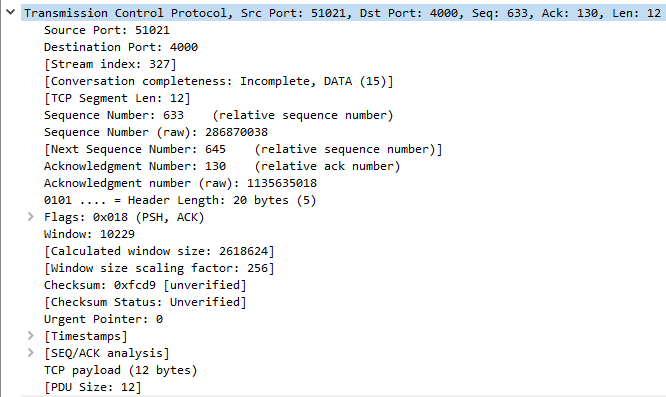
\includegraphics[width=\textwidth]{img/soluzioni_websocket-chat/wireshark-3.png}
	\end{figure}\newpage
	
	\noindent
	Adesso che è chiaro quale siano i client (quelli \dquotes{marchiati} con MASKED e il \href{https://en.wikipedia.org/wiki/WebSocket#Client_to_Server_Masking}{motivo per cui i messaggi sono mascherati è dovuto ad una questione di sicurezza}) e quale il server, è possibile vedere sulla colonna (la terza) di sinistra qual'è il tempo in cui ogni client comunica al server che è ancora vivo:
	\begin{figure}[!htp]
		\centering
		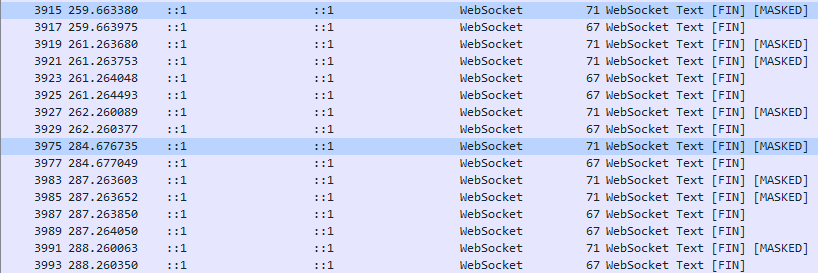
\includegraphics[width=\textwidth]{img/soluzioni_websocket-chat/wireshark-4.png}
	\end{figure}
	
	\noindent
	In questo caso, al tempo 259 il client con porta 51021 ha comunicato al server che è ancora vivo. Ovviamente il server ha risposto con un ACK e successivamente gli altri 3 client hanno comunicato al server la loro presenza. Al tempo 284, nuovamente il client con porta 51021 ricomunica al server che è ancora vivo (idem per gli altri). Si deduce che il client fa sapere al server che è ancora connesso ogni 25 secondi circa ($284-259=25$).\newline
	Documentazione ufficiale riguardo al Keep-Alive nel protocollo WebSocket: \url{https://websockets.readthedocs.io/en/stable/topics/timeouts.html}\newline
	RFC documentation: \url{https://www.rfc-editor.org/rfc/rfc6455#page-36}\newpage
	
	\noindent	
	\textcolor{Red3}{\textbf{\emph{\underline{Esercizio 2}}}}\newline
	
	\noindent
	Modificare il sorgente del codice per fare in modo che ad ogni utente connesso alla chat arrivi nella console il messaggio \dquotes{l'utente sta scrivendo...}.\newline
	
	\noindent
	NOTA: Lato client, bisogna spedire al server un evento apposito (ad es. \dquotes{typing}) quando l'utente scrive sulla tastiera (catturando l'evento di sistema \dquotes{keypress}). Lato server, la chiamata \textsf{webSocket.broadcast.emit('typing', data)} rilancia l'evento \dquotes{typing} a tutti i client connessi tranne che a quello dalla quale si è ricevuto il messaggio. Lato client infine gestire la ricezione de messaggio \dquotes{typing} che arriva dal server (si veda la gestione del messaggio \dquotes{UploadChat}).\newline
	
	\noindent	
	\textcolor{Green4}{\textbf{\emph{\underline{Soluzione esercizio 2}}}}\newline
	
	\noindent
	\lstinputlisting[language=JavaScript]{code/server_ex2.js}
	Il codice è rimasto lo stesso (paragrafo~\ref{codice Back-end server}), l'unica modifica effettuata è stata dalla riga 38 alla riga 40 in cui si impone al server di inoltrare il messaggio ricevuto, con tag \textsf{typing}, a tutti gli altri client.\newpage
	
	\noindent
	\lstinputlisting[language=JavaScript]{code/chat_ex2.js}
	Il codice del front-end è rimasto pressoché identico (paragrafo~\ref{codice Front-end JavaScript}) tranne a due modifiche importanti:
	\begin{itemize}
		\item (20-26) Sull'elemento \textsf{message} della pagina HTML, si crea un evento. Nel momento in cui una lettera viene premuta, il client invierà il messaggio con tag \textsf{typing} al server, inserendo nel payload il nome del mittente (\textsf{sender.value}).
		
		\item (50-60) Alla ricezione dell'evento \textsf{typing} da parte del server, il client stamperà la scritta \textsf{typing...} se e solo se supera il controllo alla riga 52, ovvero se non è lui il mittente (come da specifica dell'esercizio).
	\end{itemize}
	
	\longline\newline
	
	\noindent	
	\textcolor{Red3}{\textbf{\emph{\underline{Esercizio 3}}}}\newline
	
	\noindent
	Modificare a piacimento il contenuto del file \textsf{public/index.html} e valutare l'impatto grafico.\newline
	
	\noindent	
	\textcolor{Green4}{\textbf{\emph{\underline{Soluzione esercizio 3}}}}\newline
	
	\noindent
	Una modifica che è possibile fare è l'aggiunta di un altro titolo con tag h2. Ovviamente i colori saranno in tema con quelli specificati dal file CSS (styles.css).\newline
	
	\longline\newline
	
	\noindent	
	\textcolor{Red3}{\textbf{\emph{\underline{Esercizio 4}}}}\newline
	
	\noindent
	Provare a collegarsi allo stesso server da browser presenti su diversi PC collegati in rete.\newline
	
	\noindent	
	\textcolor{Green4}{\textbf{\emph{\underline{Soluzione esercizio 4}}}}\newline
	
	\noindent
	In teoria dovrebbe funzionare anche con localhost, ma non ci sono riuscito per cui non posso fornire più di tante informazioni a riguardo.\newpage
	
	\subsection{Architetture orientate ai servizi (Service-Oriented Architecture, SOA)}
	
	Solitamente le applicazioni sono monolitiche, ovvero hanno un'interfaccia utente, la quale richiama delle funzionalità fornite da una serie di librerie linkate in un unico programma che è eseguito sulla macchina dell'utente.\newline
	
	\noindent
	Al giorno d'oggi esiste un altro approccio di sviluppo delle applicazioni che riguarda SOA. Le \textcolor{Red3}{\textbf{architetture orientate ai servizi}} (\emph{Service-Oriented Architecture}) riguarda lo sviluppo di applicazioni complesse attraverso la \textbf{combinazione di diversi programmi attraverso la rete}:
	\begin{itemize}
		\item L'interfaccia utente e qualche funzionalità di base sono eseguito sull'host dell'utente.
		\item Le funzionalità principali dell'applicazione sono fornite da programmi che sono eseguiti su uno o più server.
	\end{itemize}

	\noindent
	I \textcolor{Green4}{\textbf{vantaggi}} sono molteplici:
	\begin{itemize}
		\item \textbf{Potenza di calcolo e memoria} sono delegate al server;
		
		\item \textbf{Protezione} della proprietà intellettuale su \textbf{algoritmi} strategici;
		
		\item \textbf{Annullamento} della necessità di distribuire \textbf{aggiornamenti} software quando le modifiche riguardano solo il codice dei server;
		
		\item Nuovo modello economico: \textbf{pay per use};
		
		\item \textbf{Eliminazione della pirateria}.
	\end{itemize}
	Nonostante i grandi vantaggi che propone, c'è un \textbf{requisito fondamentale} che deve essere rispettato: \textbf{la presenza e l'affidabilità della rete}.
	
	\longline
	
	\subsubsection{Funzioni remote e webservice}
	
	\noindent
	Queste architetture \textbf{si basano} completamente sui servizi offerti, ovvero sulle \textbf{funzioni remote}.
	
	Le \textcolor{Red3}{\textbf{funzioni remote}} hanno il seguente funzionamento. Il \textbf{server espone una API}\footnote{Application program interface (API): insieme delle funzioni/metodi esposte da una certa libreria.}, \textbf{la quale descrive una serie di funzioni che il client} (\underline{non} il web browser) \textbf{può invocare}. Quindi, l'implementazione effettiva del \textbf{codice si trova \emph{server-side}}, mentre il codice che richiama una funzione specifica dell'API si trova \emph{client-side}.\newline
	
	\noindent
	In passato le tecnologie utilizzate per eseguire una chiamata a funzione remota erano scritte completamente in C e venivano chiamate \emph{Remote Procedure Call} (RPC). Dopodiché, vennero semplificate e programmate in Java tramite il \emph{Java Remote Method Invocation} (JAVA RMI). Successivamente, ci fu l'invenzione del \emph{Common Object Request Broker Architecture} (CORBA) che permise di scrivere e di far comunicare più client/server con linguaggi differenti.\newline
	Al giorno d'oggi, grazie all'approdo delle \textcolor{Red3}{\textbf{webservice}}, al protocollo HTTP/HTTPS e alla metodologia REST, le cose sono molto più semplici.
	
	\longline
	
	\subsubsection{Webservice basati su REST}
	
	I webservice basati su REST hanno molteplici vantaggi. Questa metodologia consente di poter \textbf{utilizzare due linguaggi di programmazione differenti \emph{client-side} e \emph{server-side}}. Anche l'\textbf{architettura può essere differente}. Questo grazie a due componenti fondamentali:
	\begin{itemize}
		\item \textbf{Funzione STUB}, \emph{client-side}: codifica dei parametri trasmessi e la decodifica dei valori di ritorno;
		
		\item \textbf{Componente SKELETON}, \emph{server-side}: decodificare l'input, eseguire il codice della libreria, codificare l'eventuale risultato e inviarlo al client.
	\end{itemize}
	La metodologia REST utilizza il protocollo HTTP/HTTPS. Il suo \textbf{servizio principale sono le chiamate remote e per farlo utilizza l'URL}, il quale è stato mappato (\emph{mapping}).
	
	I \textbf{parametri possono essere passati tramite URL}, metodo GET, oppure dopo l'header \textbf{nel payload}, con il metodo POST o PUT.\newline
	
	\noindent
	Alcune dei metodi HTTP più famosi in base ai quali viene eseguita una funzione specifica:
	\begin{itemize}
		\item \textbf{POST}: usato da funzioni che \textbf{creano un nuovo oggetto} sul server;
		
		\item \textbf{PUT}: usato da funzioni che \textbf{aggiornano un oggetto esistente} sul server;
		
		\item \textbf{GET}: usato da funzioni che \textbf{recuperano informazioni di un oggetto} sul server;
		
		\item \textbf{DELETE}: usato da funzioni che \textbf{distruggono un oggetto esistente} sul server;
	\end{itemize}
	Solitamente i \textbf{valori di ritorno} sono sotto forma di file JSON.\newline
	
	\noindent
	I \textcolor{Green4}{\textbf{vantaggi}} sono:
	\begin{itemize}
		\item A differenza di CORBA, il \textbf{webservice utilizza il protocollo HTTP/HTTPS}. Di conseguenza, elementi come \textbf{firewall o NAT sono già predisposti all'utilizzo} senza troppe complicazioni;
		
		\item Il \textbf{debugging è facilitato} (e quindi anche lo sviluppo di applicazioni) dall'utilizzo di contenuti testuali nelle transazioni, per esempio i file JSON.
	\end{itemize}\newpage
	
	\subsubsection{Breve introduzione ai file JSON}
	
	I file \textcolor{Red3}{\textbf{JSON}} sono dei file testuali nati con JavaScript, ma ad oggi supportati da quasi tutti i linguaggi di programmazione.\newline
	
	\noindent
	La sua è una \textbf{struttura gerarchica} facilmente leggibile da un umano e parserizzabile da un programma. La sua sintassi è semplice ed è formato da coppie \dquotes{\textsf{attributo:valore}}.\newline
	
	\noindent
	Possono essere presenti anche array, rappresentati con le parentesi quadre, e strutture dati, rappresentate con le parentesi graffe. Un \textcolor{Green4}{\textbf{esempio}} di formattazione JSON:
	\begin{lstlisting}
{"impiegati":[
	{
		"nome":"Giovanni",
		"cognome":"Rossi"
	},
	{
		"nome":"Anna",
		"cognome":"Bianchi"
	},
	{
		"nome":"Pietro",
		"cognome":"Verdi"
	}
]}\end{lstlisting}
\end{document}